\documentclass[ignorenonframetext]{beamer}
%\documentclass[a4paper,12pt,titlepage]{article}
%\usepackage[hyperref]{beamerarticle}

\usepackage{graphicx}
\usepackage[utf8]{inputenc}
\usepackage{pdfpages}
\usepackage{textcomp}
\usepackage{fancyhdr,url}
\usepackage{amsmath}
\usepackage{mathtools}
\usepackage{Exercise}
\setlength{\headheight}{15pt}
\usepackage{tikz}
\usetikzlibrary{mindmap,datavisualization,shapes,arrows}
\usepackage{smartdiagram}
\usepackage{overpic}
\usepackage[version=4]{mhchem}

\mode<presentation>{
\usetheme{JuanLesPins}
\AtBeginLecture{\frame{\Large Lecture: \insertlecture}}
\usepackage[absolute,overlay]{textpos}
%\includeonlylecture{Lecture 8}
%\includeonlyframes{current}
}

\logo{\includegraphics[height=1cm]{../graphics/crac}}


\mode<article>{
\usepackage[absolute]{textpos} 
\usepackage[a4paper, top=1.5in]{geometry}
\pagestyle{fancy}
\fancyhf{}
\lhead{CM4019}
\chead{\footnotesize PHOTOCHEMISTRY}
\rhead{\thepage}
\lfoot{School of Chemistry, UCC}
\cfoot{\tiny{version 2022.01}}
\rfoot{Semester 1 2022/2023}}

\title{CM4019 -- Lasers, Photochemistry and Spectroscopy}
\subtitle{\includegraphics[height=3cm]{../graphics/colorspectrum}}
\author{Stig Hellebust \\\includegraphics[height=2cm]{../graphics/crac}}
\institute{School of Chemistry \\ University College Cork}
\date{Semester 1 2022/2023}

\renewcommand*\contentsname{}

\tikzset{
    invisible/.style={opacity=0},
    visible on/.style={alt={#1{}{invisible}}},
    alt/.code args={<#1>#2#3}{%
      \alt<#1>{\pgfkeysalso{#2}}{\pgfkeysalso{#3}} % \pgfkeysalso doesn't change the path
    },
  }

\begin{document}
\mode<article>{\maketitle \tableofcontents}

\begin{frame}
	\titlepage
\end{frame}

\newpage

\section*{Scope of this document}
This document contains \emph{all} the material relevant to the photochemistry section of the CM4019 Exam, \emph{including} directed study material. What that means is that everything that is covered in the lectures is contained in this document, and some additional material not covered by lectures, which makes up the directed study section. 

In other words, this is the only document that is mandatory reading. But the optional reading material provided separately is recommended to assist your understanding of the material.

The problems and exercises at the end will help prepare you for the exam questions, so make sure you can solve them.

\section{Introduction}

\lecture{Intro and Terminology}{Lecture 1}

\begin{frame}[<+->]
\frametitle{What is photochemistry?}
\begin{enumerate}
\item Light interacts with electrons in atoms and molecules
\item Chemical bonds depend on electrons
\item Chemical reactions involve braking and forming of bonds
\item Light causes chemical reactions by interfering with the electron structure
\end{enumerate}
\end{frame}

\begin{frame}
  \begin{center}
     \includegraphics[width=12cm]{../graphics/colorspectrum}
  \end{center}
\end{frame}

\begin{frame}
  \begin{center}
     \includegraphics[width=12cm]{../graphics/sunglasses}
  \end{center}
\end{frame}

\begin{frame}
  \begin{center}
     \includegraphics[width=12cm]{../graphics/sharks}
  \end{center}
\end{frame}
	
\section{Basic concepts}

\begin{frame}[<+->]
\frametitle{Terminology and basic concepts}
  \begin{itemize}
  \item Photochemistry
  \item Excited state of a molecule
  \item Jablonski-state diagram
  \item Singlet and Triple excited states
  \item Spin selection rules
  \item Absorbance
  \item Vibrational relaxation
  \item Internal conversion
  \item Fluorescence
  \item Inter-system crossing
  \item Phosphorescence
  \item[] \fcolorbox{black}{green}{\textcolor{black}{\parbox{.9\textwidth}{\textbullet \enspace The competing processes that can occur after absorption \enspace of a photon\\
	\textbullet \enspace The allowed and forbidden spin transitions}}}
  \end{itemize}
\end{frame}

\begin{frame}
\frametitle{Motivation}
\textbullet Converting solar energy to chemical energy\medskip\\
\textbullet Use the energy in sunlight to convert water to hydrogen gas\medskip\\
\textbullet The Hydrogen can be used as a ``solar fuel''\medskip\\

\url{https://www.youtube.com/watch?v=PdmHH6KY_Qs}
\end{frame}

\begin{frame}
 \begin{description}
  \item[Photochemistry:] Photochemistry is concerned with the chemical effects of light. Generally, this term is used to      describe a chemical reaction caused by absorption of ultraviolet (\(\lambda\) = 100-400 nm), visible light (\(\lambda\) = 400-750 nm) or infrared radiation (\(\lambda\) = 750-2500 nm)
  \item[Excited state of a molecule:] Energy of the molecule has increased by the energy of the absorbed photon \\
  
 \end{description}
\end{frame}

The normal electronic configuration of any molecule is called the \textbf{ground state}. Energy from absorbed light is used to promote an electron from the highest occupied molecular orbital (HOMO) of the ground state (\(\psi_2\)) into the lowest unoccupied molecular orbital (LUMO) of the excited state (\(\psi_3^*\)). A species with a promoted electron is called an \emph{excited state}. The \(\psi_3^*\) becomes the HOMO of the excited state. \emph{The HOMOs of the ground state and the excited sate have opposite symmetries.}

%draw energy diagram here (Fig 25.6 in Marc Loudon Org Chem)

\begin{frame}
\[ E_{exc} = E^* - E_0 = h\nu = hc/\lambda \]  
  \begin{description}
    \item[\(E_{exc}\)] Electronic excitation energy
    \item[\(E^*\)] Energy of the excited state		
    \item[\(E_0\)] Energy of the ground state
    \item[\(h\)] Planck’s constant
    \item[\(\nu\)] Frequency of absorbed radiation
    \item[	\(c\)] Speed of light
    \item[	\(\lambda\)] Wavelength of absorbed radiation
  \end{description}
\end{frame}

\subsection{Singlet and Triplet excited states}

\begin{frame}
	\frametitle{Singlet and Triplet excited states}
	When an electron in a molecule with a singlet ground state is excited (via absorption of radiation) to a higher energy level, 		either an excited singlet state or an excited triplet state will form
	\begin{center}
	\includegraphics[width=\textwidth]{../graphics/excitedstates}
	\end{center}
\end{frame}

\begin{frame}
	\begin{alertblock}{Excited states}
	\begin{itemize}
		\item An excited singlet state is a molecular electronic state such that all electrons are paired. Multiplicity is 1
		\item In an excited triplet state the excited electron is no longer paired with the ground state electron; that is, they are 			  parallel (same spin). Multiplicity is 3
	\end{itemize}
	\end{alertblock}
\end{frame}

\subsection{The Jablonski-state diagram}

\begin{frame}
	\frametitle{The Jablonski-state diagram}
	\begin{itemize}
		\item The dynamics of a photochemical reaction can be considered statistically
		\item Several competing processes can occur after absorption of a photon and are \emph{unimolecular physical decay 			reactions}
		\item The most important are:
			\begin{columns}[t]
				\column{.5\textwidth}
					\begin{block}{Radiative processes}
						\begin{itemize}
							\item Fluorescecnce decay
							\item Phosphorescence decay
						\end{itemize}
					\end{block}
				\column{.5\textwidth}
					\begin{block}{Non-radiative processes}
						\begin{itemize}
							\item Intersystem crossing between Singlet-Triple (S-T) manifolds
							\item Internal conversion to lower excited states
							\item Radiationless decay to ground state
						\end{itemize}
					\end{block}
			\end{columns}

	\end{itemize}
\end{frame}
		
\begin{frame}
	\frametitle{The Jablonski-state diagram}
	\parbox{\textwidth}{\emph{The Jablonski-state diagram} is essentially a summary of the possible processes that can 					occur upon 	\emph{electronic excitation}}
	\includegraphics[width=\textwidth]{../graphics/jablonski_1D}
	\begin{itemize}
		\item \emph{Straight lines} show the conversion between a photon of light and the energy of an electron 							(\emph{radiative})
		\item \emph{Curved lines} show transitions of electrons without interaction with light (\emph{non-radiative})
	\end{itemize}
\end{frame}

\subsection{multiplicity}

\begin{frame}
	\frametitle{Multiplicity}
	Singlet and triplet states have different \emph{multiplicity} \\
	
	The multiplicity of and energy level is defined as \textbf{2S + 1}, where S is the \emph{total spin angular momentum} \newline
	
	\LARGE Spin selection rules:\newline \normalsize
	An electronic transition is allowed by the spin selection rule only if the multiplicity of the initial and final states are 				identical, \textit{e.g.} \newline
	\begin{center} \fbox{
\begin{tabular}{c c c}
	S \(\rightarrow\) S & T \(\rightarrow\) T &  are \alert{allowed}\\
	S \(\rightarrow\) T & T \(\rightarrow\) S &  are \alert{forbidden}
	\end{tabular} }
	\end{center} 
\end{frame}

\subsection{Absorbance}

\begin{frame}[shrink=10]
\frametitle{Absorbance}
\begin{columns}[onlytextwidth]
\begin{column}{.3\textwidth}
	\includegraphics[height=3in]{../graphics/absorbance}
\end{column}
%\begin{column}{.1\textwidth}
%\end{column}
\begin{column}{.6\textwidth}
			\begin{itemize}
				\item \fbox{\parbox{\linewidth}{\textcolor{purple}{Absorbance (purple arrows)} is the method by which an electron is excited from a 											lower energy level to a higher energy level}}
				\item The transition will usually occur from the loweest (ground) electronic state (\(S_0\)) due to the 								statistical mechanical issues of most electrons occupying a low lying state at reasonable temperatures
				\item Absorbance is a very fast transition, on the order of \emph{\(10^{-15}\) seconds}
				\item As excitation to a triplet state involves a ``forbidden'' spin transition, it is less probable when the 							molecule absorbs radiation
			\end{itemize}
\end{column}
\end{columns}
\end{frame}
	
\subsection{Vibrational relaxation}

\begin{frame}
\frametitle{Vibrational relaxation}
\begin{columns}[onlytextwidth]
\begin{column}{.3\textwidth}
		\includegraphics[height=2.5in]{../graphics/vibrelax}
\end{column}
\begin{column}{.6\textwidth}
			\begin{itemize}
				\only<1>{\item \fbox{\parbox{\textwidth}{\textcolor{blue}{Vibrational relaxation (blue arrows)} is where energy deposited 							by a photon into the electron is given away to other vibrational modes as kinetic energy, \textit{i.e.} a 							non-radiative process}}
				\item This relaxation occurs between vibrational levels, so generally electrons will not change from one 								electronic level to another}
				\only<2->{\item This kinetic energy may stay within the same molecule, or it may be transferred to other molecules 							around the excited molecule, largely depending on the phase of the probed sample}
				\only<2->{\item For example, vibrational relaxation will occur within an electronic state in condensed phases and in gas 						phases in the presence of a 3rd body}
				\only<2->{\item This process is also very fast transition, on the order of \emph{\(10^{-11}\) to \(10^{-14}\) seconds}}
			\end{itemize}
\end{column}
\end{columns}
\end{frame}
	
\subsection{Internal conversion}

\begin{frame}
\frametitle{Internal conversion}
\begin{columns}[onlytextwidth]
\begin{column}{.3\textwidth}
			\includegraphics[height=2.5in]{../graphics/internconv}
\end{column}
\begin{column}{.1\textwidth}
\end{column}
\begin{column}{.6\textwidth}
			\begin{itemize}
				\only<1>{\item \fbox{\parbox[b]{\textwidth}{\textcolor{green}{Internal conversion (green arrows)} is the \emph{non-								radiative} transition of an electron between two states of the \emph{same multiplicity} (\(\Delta S = 0 							\)) and \emph{same energy}}}
				\item Internal conversion occurs because of the overlap of vibrational and electronic energy states
				\item At energy levels grater than \(S_1\), the manifold of vibrational energy levels strongly overlap with the 						electronic energy levels}
				\only<2>{\item This overlap gives a higher degree of probability that the electron can transition between vibrational 							levels that will lower the electronic state, and is fast (on the order of \emph{\(10^{-6} to 10^{7}\) 							seconds}
				\item Due to a lack of vibrational and electronic energy state overlap and large energy difference, internal 							conversion is slow (\emph{\(10^{-6}\) to \(10^{-7}\) seconds}) between \(S_0\) and \(S_1\)}
			\end{itemize}
\end{column}
\end{columns}
\end{frame}

\subsection{Fluorescence}

\begin{frame}
\frametitle{Fluorescence}
\begin{columns}[onlytextwidth]
\begin{column}{.3\textwidth}
		\includegraphics[height=2.5in]{../graphics/fluorescence}
\end{column}
\begin{column}{.1\textwidth}
\end{column}
\begin{column}{.6\textwidth}
			\begin{itemize}
				\only<1>{\item \fbox{\parbox[b]{\linewidth}{\textcolor{red}{Fluorescencce (red arrow)} is an \emph{emissive 						pathway} between two levels of the \emph{same multiplicity} (\(\Delta S = 0\)) but \emph{different 						energy}, e.g. \(S_1 \rightarrow S_0\) in organic molecules}}
				\item Fluoresence is a slow process, on the order of \(10^{-7} to 10^{-9}\) seconds}
				\only<2>{\item Fluorescence is most often observed between the \(S_1\) and \(S_0\) as at higher energies it is more 							likely that energy will be dissipated through internal conversion and vibrational relaxation
				\item The energy of fluorescent photons is almost always less than that of the exciting photons
				\item The difference is because energy is lost in internal conversion and vibrational relaxation, where it is 							transferred away from the electron}
			\end{itemize}
\end{column}
\end{columns}
\end{frame}

\subsection{Intersystem crossing}

\begin{frame}
\frametitle{Intersystem crossing}
\begin{columns}[onlytextwidth]
\begin{column}{.3\textwidth}
		\resizebox{!}{2in}{\includegraphics{../graphics/intersystem}}
		%\includegraphics[width=3in]{../graphics/intersystem}
\end{column}
\begin{column}{.1\textwidth}
\end{column}
\begin{column}{.4\textwidth}
			\begin{itemize}
				\only<1>{\item[] \fbox{\parbox[b]{\textwidth}{\textcolor{brown}{Intersystem crossing (ISC, brown arrow)} is the 					\emph{non-radiative} transition of an electron between two states of \emph{different multiplicity}  (\( 							\Delta S \ne 0 \) ) but the \emph{same energy}}}
				\item During ISC the electron changes spin multiplicity from ad excited singlet state to an excited triplet 						state, \textit{e.g.} \(S_1\) to \(T_1\)}
				\only<2>{\item Technically, ISC is a forbidden transition, \textit{i.e.} a transition that based strictly on electronic 								selection rules should not happen
				\item Thus, the time scale of ISC is on the order of \emph{\(10^{-4} to 10^{-7}\) seconds}, one of the 								slowest forms of relaxation}
			\end{itemize}
\end{column}
\end{columns}
\end{frame}

\subsection{Phosphorescence}

\begin{frame}
\frametitle{Phosphorescence}
\begin{columns}[onlytextwidth]
\begin{column}{.3\textwidth}
		\resizebox{!}{2in}{\includegraphics[height=3in]{../graphics/phosphor}}
\end{column}
\begin{column}{.1\textwidth}
\end{column}
\begin{column}{.4\textwidth}
			\begin{itemize}
				\only<1>{\item[] \fbox{\parbox[b]{\textwidth}{\textcolor{pink}{Phosphorescence (pink arrow)} is an \emph{emissive 								pathway} between two levels of \emph{different multiplicity}  (\(\Delta S \ne 0 \) ) and \emph{different 						energy}, e.g. \(T_1 \rightarrow S_0\) in organic molecules}}}
				\only<2>{\item Since a transition in spin multiplicity is observed, phosporescence is another manifestation of ISC
				\item Thus, the time scale of phosphorescence is on the order of \emph{\(10^{-3}\) seconds}}
			\end{itemize}
\end{column}
\end{columns}
\end{frame}

\begin{frame}[shrink]
\frametitle{Summary of competing processes that can occur after absorption of a photon}
\begin{center}
	\begin{tabular}{p{0.2\textwidth}| p{0.15\textwidth} |p{0.13\textwidth}| p{0.1\textwidth}| p{0.15\textwidth} |p{0.2\textwidth}}
	\textbf{Process} & \textbf{Non-radiative or emissive pathway} & \textbf{State change} & \textbf{Energy change} & \textbf{Multi\-plicity change} & \textbf{Time-scale (seconds)}\\\hline\\ 
	Vibrational relaxation & Non-radiative & No & Yes & No \newline (\(\Delta S = 0\)) & \(10^{-11} to 10^{-14}\)\\ \hline
	Internal conversion & Non-radiative & Yes, \textit{e.g.} \newline \(S_2 \rightarrow S_1\) \newline \(T_2 \rightarrow T_1\) \newline \(S_1 \rightarrow S_0\) & No & No \newline (\(\Delta S = 0 \)) & \(10^{-11} to 10^{-14}\) \newline for \(S_n \rightarrow S_1\) \newline  and \(T_n \rightarrow T_1\); \(10^{-6}\) to \(10^{-7}\) \newline for \(S_1 \rightarrow S_0\) \\ \hline
	Fluorescence & Emissive & Yes, \textit{e.g.} \newline \(S_1 \rightarrow S_0\) & Yes & No \newline (\(\Delta S = 0\)) & \(10^{-7}\) to \(10^{-9}	\) \\ \hline

	Intersystem crossing & Non-radiative & Yes, \textit{e.g.} \newline \(S_1 \rightarrow T_1\) & No & Yes \newline (\(\Delta S \ne 0\)) & \(10^{-4}\) to \(10^{-7}\)\\ \hline
	Phosphor\-escence & Emissive & Yes, \textit{e.g.} \newline \(T_1 \rightarrow S_0\) & Yes & Yes \newline (\(\Delta S \ne 0\)) & \(>10^{-3}\) \\ 
	\end{tabular}
\end{center}
\end{frame}

\subsection{spin transitions}

\begin{frame}
\frametitle{Summary of allowed and forbidden spin transitions}
\begin{center}
\includegraphics[width=\columnwidth]{../graphics/transitionsummary}
\end{center}
\end{frame}
	
\lecture{The absorption process}{Lecture 2}

\section{The absorption process}
	\begin{frame}
	\frametitle{Lecture contents}
		\begin{itemize}
			\item The absorption process
			\item The Jablonski-state diagram
			\item 2-D configuration co-ordinate Jablonski diagram
			\item Basic Laws of photochemistry
			\item Quantum yields (Efficiency of photon usage)
			\item The Frank Condon Principle
		\end{itemize}
	\end{frame}
	
\begin{frame}[<+->]
\frametitle{The absorption process}
\begin{itemize}
\item The absorption process is the process by which light interacts with matter to create an excited state
\item Generally in photochemistry we use \textit{\underline{electromagnetic radiation}} to create excited electronic state of molecules
\item Then \textit{\underline{photochemical}} (dissociation, isomerization) or \textit{\underline{photophysical}} (luminescence, etc.) processes subsequently occur
\item Our picture of wave-like properties is due to Maxwell, where light can be thought of as a transverse plane involving \textit{\underline{electric and magnetic fields aligned at \(90^\circ\)}} to each other
\end{itemize}
\end{frame}

\begin{frame}{electromagnetic radiation}
\includegraphics[height=3in]{../graphics/emwave}
\end{frame}
	

\begin{frame}[allowframebreaks]
\frametitle{Radiation and scattering}
\begin{itemize}
\item {\color{red}{Electromagnetic radiation}} causes electrons to be set into oscillation by the electric vector of the wave
\item If the energy does not correspond to the energy difference between two stationary states of the atom the duration of the interaction is of the order of \(\approx 10^{-14}\) seconds and phenomena such as \textit{\underline{Ralyleigh scattering}} take place
\item[] \includegraphics[height=2in]{../graphics/rayleigh}
\item Rayleigh scattering occurs when the radius of the scattering object (e.g. an atom) is much smaller than the wavelength of light 
\end{itemize}
\end{frame}

\begin{frame}
\begin{itemize}
\item However, the \textbf{\underline{wave-particle duality}} of light should not be forgotten
\item The \(19^{th}\) century pure wave theory of light is an oversimplification
\item The energy of a beam of light comes in finite chunks rather than being spread smoothly throughout a region of space
\item Thus, electromagnetic radiation is viewed as a stream of \textit{\underline{discrete particles of energy}} called \textbf{\color{red}photons}
\item In essence, a photon can be thought of as a particle with energy but \textit{\underline{no mass}}
\end{itemize}
\url{https://upload.Wikimedia.org/wikipedia/commons/e/e4/Wave-particle_duality.ogv} \newline
\url{https://en.wikipedia.org/wiki/Wave\%E2\%80\%93particle_duality}
\end{frame}

\vspace{1in}

\begin{frame}[allowframebreaks]
\frametitle{Absorption conditions}
\fbox{Absorption can occur if: \colorbox{yellow}{\textcolor{black}{\(E_{exc} = E^* - E_0 = h\nu = hc/\lambda\)}}}

\begin{description}
\item[\(E_{exc}\)] Electronic excitation energy
\item[\(E^*\)] Energy of the excited state
\item[\(E_0\)] Energy of the initial state
\item[h] Planck's constant
\item[\(\nu\)] Frequency of absorbed radiation
\item[c] Speed of light
\item[\(\lambda\)] Wavelength of absorbed radiation
\end{description}

\begin{itemize}
\item[ ] \includegraphics[height=2in]{../graphics/absorption}
\item Energy of the molecule has increased by the energy of the absorbed photon
\item An oscillating electric dipole in the atom is obtained in the direction of the electric vector of the wave
\end{itemize}

\end{frame}

\begin{frame}
\frametitle{The Jablonski-State diagram}
\begin{itemize}
\item[] \includegraphics[width=\linewidth]{../graphics/jablonski_1D}
\item Discussed in Lecture 1
\item This 1-D representation of the Jablonski diagram shows \textit{\underline{energy differences only}}
\end{itemize}
\end{frame}

\begin{frame}
\frametitle{2-D configuration co-ordinate Jablonski diagram}
\centering
\begin{figure}[h!]
\includegraphics[width=\linewidth]{../graphics/2Djablonski}
\caption{This 2-D representation of the Jablonski diagram shows \textit{\underline{energy and geometry changes}}, \textit{i.e.} shape changes due to bonds extending or changing angle}
\end{figure}
\end{frame}

\begin{frame}
\frametitle{2-D Jablonski diagram}
\begin{figure}[h!]
\includegraphics[width=\linewidth]{../graphics/2Djablonski2}
\caption{\fcolorbox{black}{yellow}{\textcolor{black}{\parbox{\textwidth}{Note that IC and ISC occur with no change in energy!}}}}
\end{figure}
\end{frame}


\subsection{Basic laws of photochemistry}

\begin{frame}
\frametitle{Basic Laws of photochemistry}
\begin{columns}[onlytextwidth]
\begin{column}{.7\textwidth}
\begin{description}
\only<1>{\item[The Grotthus-Draper Law] aka the \(1^{st}\) Law of Photochemistry. Only light which is absorbed by a molecule can be effective in producing chemical change in a molecule}
\item[The Stark-Einstein Law] \begin{itemize}
			\item[] aka the ``Law of Photochemical Equivalence Law'' 
			\item Absorption of light by a molecule is a one quantum process
			\item[\(\Rightarrow\)] This leads to the concept of \textit{\underline{Quantum yield}}, \(\Phi\)
			\end{itemize}
\end{description}
\end{column}
\begin{column}{.3\textwidth}
\only<1>{\resizebox{\linewidth}{!}{\includegraphics{../graphics/grotthus}}\\}
\resizebox{\linewidth}{!}{\includegraphics{../graphics/stark}}
\end{column}
\end{columns}
\only<2>{\textbullet \enspace The Stark-Einstein Law assumes that the excited state lifetimes are short and that the intensity of light is low. Exceptions to the rule are found in various laser-initiated photochemical reactions}
\end{frame}

\subsection{Quantum yields}

\begin{frame}
\frametitle{Quantum yields (Efficiency of photon usage)}
\begin{itemize}
\only<1>{\item The quantum yield (\(\Phi\)) is the fraction of molecules undergoing a particular photochemical/photophysical process
\[ \Phi = \frac{\textit{ rate of the process of interest}}{\textit{ rate of absorption of photons}} \]
\item In other words, the sum of the unimolecular, primary process quantum yields must be unity}
\only<2>{\item For a \emph{\underline{photochemical process}}:
\[ \Phi^\lambda = \frac{\textit{No. of moles(molecules) produced / unit vol. / unit time}}{\textit{No. of einsteins (photons) absorbed/unit vol./unit time}} \]
\item[]
\[ \Phi\lambda = \frac{\textit{Rate of formation}}{I_a} \]
where \(I_a\) = no. photons absorbed/unit volume/unit time and 1 Einstein = 1 mole of photons}
\only<3>{\small \item For a \textit{\underline{luminescence}} process:
\[ \Phi_F \ or\  \Phi_P = \frac{\textit{No. quanta emitted}}{\textit{No. quanta absorbed}} = \frac{\textit{rate of emission of luminescence}}{\textit{rate of absorption}} \] }

\only<4>{\item For example:
	\[A + h\nu \rightarrow A^*\]
	\[A^* \rightarrow A + \mathbf{\color{red}{h\nu_F}}\]
	\[Rate = - \frac{d[A]}{dt} = \frac{d[A^*]}{dt} = I_a \] 
	
	\item \(I_a\) = no. photons absorbed/unit volume/unit time
	\item \(I_a\) can be calculated by defining \(I_a = (I_0 - I_{trans})\) and knowing the volume irradiated
	\item \(I_0\) is the incident light intensity and \(I_{trans}\) is the light intensity transmitted, \( \Phi_F = \frac{k_F[A^*]}{I_a} \), where \(k_F\) is the rate coefficient of fluorescence
	\item \color{red}{\(h\nu_F\)} is the \emph{fluorescence!}}
\end{itemize}
\end{frame}

\begin{frame}
\frametitle{Quantum yields and wavelength-dependence}
\begin{columns}[T]
\begin{column}{.7\textwidth}
\begin{itemize}
\item<1-> It is important to specify the wavelength (\(\lambda\)) for quantum yields of reaction as the observed chemistry is often wavelength-dependent
\item[Q:]<2-> Are quantum yields of fluorescence (\(\Phi_F\)) in solution wavelength-dependent?
\item<3-> \(\Phi_F\) is wavelength-dependent
\item<4-> Fluorescence always starts from \(\nu = 0\) irrespective of the excitation wavelength
\item<5> This is because vibrational relaxation occurs quicker than fluorescence
\end{itemize}
\end{column}
\begin{column}{.3\textwidth}
\only<1,5>{\resizebox{1.5in}{!}{\includegraphics{../graphics/fluorescence}}}
\end{column}
\end{columns}
\end{frame}

\begin{frame}[<+->]
\frametitle{The Franck Condon Principle}
\begin{itemize}
\item Since electronic transitions are \textit{\underline{very fast compared with nuclear motions}}, vibrational levels are favoured when they correspond to a minimal change in the nuclear coordinates
\item In other words, because electronic transitions are essentially instantaneous (\(\approx10^{-15}\) seconds) there is little or no geometry change in the molecular system
\item As a result, \textit{\underline{optical transitions}} on the 2-D Jablonski diagram are \newline \textit{\underline{represented by lines of length h\(\nu\)}} \textemdash nuclei do not move in the interim
\end{itemize}
\end{frame}

\begin{frame}[shrink,label=FranckCondonL2]
\frametitle{The Franck Condon Principle}
\begin{columns}[onlytextwidth]
\begin{column}{.3\linewidth}
\begin{figure}[h!]
\includegraphics[width=\columnwidth]{../graphics/FC1}
\caption{\footnotesize Franck-Condon principle energy diagram. The potential wells are shown favouring transitions between \(\nu = 0\) and \(\nu = 2\)}
\end{figure}
\end{column}
\begin{column}{.7\linewidth}
\fbox{\parbox{\linewidth}{\small The \emph{Frank Condon Principle} states that during an electronic transition, a change from one vibrational energy level to another will be more likely to happen if the \emph{\underline{two vibrational wave functions overlap}} more significantly }}
\begin{figure}[h!]
\includegraphics[width=\columnwidth]{../graphics/FC2}
\end{figure}
\end{column}
\hyperlink{FranckCondonL4<5>}{\beamerreturnbutton{L4}}
\end{columns}
\end{frame}

\begin{frame}
\frametitle{Quantum yield example}
\begin{example}
In the chemical reaction \ce{A ->[h\nu] 2B + C}, the quantum yield, \(\Phi_{500nm} = 2.1\times 10^2\ mol\ Einstein^{-1}\)\\\hspace{3pt}

We started with 300 mmol of A and ended up with 2.28 mmol of B. We will calculate how many photons were absorbed in the reaction.\\
\medskip \(\Phi = \frac{moles\ reacted}{moles\ absorbed} = 2.1\times 10^2\)\\
Remember, one mole reacted gives two moles of product.\\
\medskip \begin{multline*}moles\ absorbed\ = \frac{1}{2} *\frac{2.28\times 10^{-3}}{2.1\times 10^2} = 5.43\times 10^{-6}\ Einstein\\ \xRightarrow{\times 6.022\times10^{23}} 3.3\times 10^{18}\ photons\end{multline*}
\end{example}
\end{frame}

\begin{frame}
\frametitle{What you have learnt to do in this lecture}
\begin{itemize}
\item Draw a 2-D Jablonski diagram
\item Illustrate the following processes using the diagram: Absorption, Internal Conversion, Vibrational Relaxation, Interystem Crossing, Fluorescence and Phosphorescence
\item Calculate quantum yields for a photochemical or photophysical process
\end{itemize}
\end{frame}

\lecture{Absorption to emission 1: Fluorescence, internal conversion and the singlet state}{Lecture 3}

\section{Fluorescence, internal conversion and the singlet state}
	\begin{frame}
	\frametitle{Lecture contents}
		\begin{itemize}
			\item Absorbance (the Franck Condon Principle)
			\item Kasha's rule
			\item Internal conversion and the singlet state
			\item Fluorescence 
			\item "Mirror symetry" of absorption and fluorescence spectra
			\item Fluorescence quenching
			\item Kinetics of fluorescence: the Stern-Volmer relationship
			\item Stern-Volmer plots
		\end{itemize}
	\end{frame}

\subsection{The Frank-Condon principle}
\begin{frame}[label=FranckCondonL4]
\frametitle{Franck-Condon Principle (absorption)}
\only<1-3>{At low temperatures (in effect the typical temperature most researchers work at), the electrons in the molecule \emph{\underline{start out in the \(\nu=0\) vibrational level}} of the ground electronic state
\begin{columns}[onlytextwidth,T]
\begin{column}{.5\textwidth}
\includegraphics[height=1.8in]{../graphics/franck1}
\end{column}
\begin{column}{.45\textwidth}
\color{red} \bfseries
\only<1>{ upon absorbing a photon, the electrons make a transition to the excited electronic state}
\only<2>{ On average, the \emph{\underline{transition energy is larger}} than the difference between the lowest vibrational level of the ground state (v" = 0) and the lowest vibrational level of the excited state (v'=0), known as the \emph{\underline{zero-zero (0-0) transition energy}} }
\only<3>{ Thus, the excited electron can \emph{end up in any of a number of vibrational levels} in the excited state}
\end{column}
\end{columns} }
\only<4->{
\mode<presentation>{\begin{textblock}{6}(1,4)}
\begin{figure}
\includegraphics[height=1.7in]{../graphics/franck2}
\caption{Franck-Condon principle energy diagram. The potential wells are shown favouring transitions between v"=0 and v'=2}
\end{figure}
\mode<presentation>{\end{textblock}}}
\only<4>{
\mode<presentation>{\begin{textblock}{6}(8,4)}
The \textbf{Franck-Condon principle} states that the rapid absorption of light by a molecule (\(10^{-15}\)s is too fast to permit any significant motions of the nuclei in the molecule or in the solvent molecules surrounding it\break
\mode<presentation>{\end{textblock}}}
\only<5>{
\mode<presentation>{\begin{textblock}{6}(8,4)}
The \emph{\underline{probability}} that the molecule can end up in any particular vibrational level is proportional to the square of the (vertical) overlap of the vibrational wavefunctions of the original and the final state
\hyperlink{FranckCondonL2<1>}{\beamergotobutton{L2}}
\mode<presentation>{\end{textblock}}}
\end{frame}	

\begin{frame}[t]
\frametitle{Franck-Condon principle cont/d}
\only<1>{\textbullet \quad Thus, the transition that results in fluorescence occurs from the \emph{lowest vibrational level of the excited state}\newline
\textbullet \quad On average, the transition energy is \emph{less} than the zero-zero (0-0) transition energy}
\mode<presentation>{\begin{textblock}{7}(0,7)}
\includegraphics[height=6\TPHorizModule]{../graphics/franck3}
\mode<presentation>{\end{textblock}}
\mode<presentation>{\begin{textblock}{8}(8,7)}
\only<1>{\textcolor{red}{ \textbullet \enspace Thus, the emitted electron can \emph{end up in any of a number of vibrational levels} in the ground state}}
\only<2>{\textcolor{red}{ \textbullet \enspace The energy of fluorescent photons is almost always less (i.e. red-shifted) than that of the exciting photons}}
\only<3>{\textbullet \enspace \textcolor{red}{This difference is because energy is lost in internal conversion and vibrational relaxation, where it is transferred away from the electron (Kasha's rule)}}
\mode<presentation>{\end{textblock}}
\end{frame}

\subsection{Kasha's rule}
\begin{frame}[t]
\frametitle{Kasha's rule}
Kasha's rule states that in the electronic excited state molecules quickly relax to the \emph{\underline{lowest vibrational level of the lowest electronic excitation state}}
\mode<presentation>{\begin{textblock}{8}(0,7)}
\includegraphics[width=8\TPHorizModule]{../graphics/kasha}
\mode<presentation>{\end{textblock}}
\mode<presentation>{\begin{textblock}{7}(8,7)}
Fluorescence is much slower than internal conversion and vibrational relaxation\break
\begin{tabular}{p{2.5\TPHorizModule} p{3.5\TPHorizModule}}
\textbf{Process} & \textbf{Time-scale \-(seconds)} \\\hline\hline
Vibration relaxation & \(10^{-11}\) to \(10^{-14}\)\\\hline
Internal conversion &	\(10^{-11} \) to \(10^{-14}\) for \( S_n \rightarrow S_1\)\\\hline
Fluorescence & \(10^{-7}\) to \(10^{-9}\)\\\hline
\end{tabular}
\mode<presentation>{\end{textblock}}
\end{frame}

\subsection{Internal Conversion}
\begin{frame}[t]
\frametitle{Internal Conversion}
\fbox{\parbox{10\TPHorizModule}{\textcolor{green}{Internal Conversion (IC, green arrow)} is the \emph{non-radiative} transition of an electron between two states of the \emph{same multiplicity} (\(\Delta S=0\)) and \emph{same energy}}}\par
\medskip
\onslide<2->{\parbox{10\TPHorizModule}{\textcolor{red}{Kasha's rule} states that in the electronic excited state molecules quickly relax to the \emph{lowest electronic excitation state} \par\smallskip
Kasha's rule is a consequence of the occurrence of internal conversion after the absorption of a photon by a molecule}}\par\medskip
\onslide<3->{\parbox{\textwidth}{\(S_2 \rightsquigarrow S_1\) internal conversion is \emph{very much faster} than the corresponding \(S_1 \rightsquigarrow S_0\) process (\(10^{12} - 10^{13} \ s^{-1}\) vs. \(10^6\ s^{-1}\)) \textbf{\color{red} WHY?}}}
\mode<presentation>{\begin{textblock}{4}(12,3)}
\includegraphics[width=4\TPHorizModule]{../graphics/internconv}
\mode<presentation>{\end{textblock}}
\end{frame}

\begin{frame}[t]
\frametitle{Franck-Condon overlaps}
The origin is the large "Franck-Condon overlap" between \(S_2\) and \(S_1\) that results from their similar energies vs. the small "Franck-Condon overlap" between \(S_1\) and \(S_0\) that results from the widely different energies\par\bigskip
\begin{tabular}{l c c}
\textbf{Compound} 	& \(S_2 - S_1\) \(\Delta E\) / cm\(^{-1}\)	&	\(S_1 - S_0\) \(\Delta E\) / cm\(^{-1}\)\\\hline
Benzene	&	9,600	&	38,400\\
Naphtalene	&	2,800	&	32,200\\\hline
\end{tabular}

\onslide<2->{\bigskip\textbullet \quad The Franck-Condon factor controls the \emph{probability} of the transition:}\newline
\onslide<3>{\textbullet \quad  \(S_n(v=0) \rightarrow S_{n-1}(v=m)\), \textit{i.e.} the transition from the lowest vibrational level of one electronic state to a high enough vibrational level of the next lower electron state \emph{such that it has the same energy} as \(S_n(v=0)\)}
\end{frame}

\begin{frame}[t]
\frametitle{Energies}
\only<1>{
\mode<presentation>{\begin{textblock}{6}(0,3)}
\includegraphics[width=5.5\TPHorizModule]{../graphics/vibwaves}
\mode<presentation>{\end{textblock}}
\mode<presentation>{\begin{textblock}{8}(6,3)}
\includegraphics[width=9.5\TPHorizModule]{../graphics/vibwaves2}
\mode<presentation>{\end{textblock}}
}
\only<2->{
When states (\textit{e.g.} \(S_1\) and \(S_2\)) are very far apart in energy, vibrational wavefunction overlap is limited - \emph{"small Franck-Condon overlap"}\newline
\begin{center} \(\implies\) Slow rate of IC, small \(k_{IC}\)\newline
Diminished rate of fluorescence, small \(k_F\)
\end{center}
}
\only<3> {
When states (\textit{e.g.} \(S_1\) and \(S_2\)) are close together in energy, more vibrational wavefunction overlap takes place and non-radiative transport is much easier - \emph{"large Franck-Condon overlap"}\newline
\begin{center} \(\implies\) Fast rate of IC, large \(k_{IC}\) \newline
Enhanced rate of fluorescence, large \(k_F\)
\end{center}
}
\end{frame}

\subsection{Fluorescence}

\begin{frame}
\frametitle{Fluorescence}
\onslide*<1-2>{\fbox{\parbox{\textwidth}{\textbullet \quad \textcolor{red}{Fluorescence (red arrow)} is an \emph{\underline{emissive pathway}} between two levels of the \emph{\underline{same multiplicity}} (\(\Delta S=0\)) but \emph{\underline{different energy}}, \textit{e.g.} \(S_1 \rightarrow S_0\) in organic molecules}}\par\bigskip }
\onslide*<1>{\includegraphics[height=2in]{../graphics/fluorescence} }
\onslide*<2>{\parbox{\textwidth}{\textbullet \quad Fluorescence does \textbf{\underline{\textit{not}}} necessarily involve singlet state intermediary\break
\textbullet \quad For example, triplet-to-triplet or quartet-to-quartet transitions would also be fluorescence}}
\end{frame}

\begin{frame}[t]
\frametitle{Mirror symmetry}
\only<1>{
\textbullet \quad The Franck-Condon principle is applied equally to absorption and to fluorescence\newline
\textbullet \quad The applicability of the Franck-Condon principle in both absorption and fluorescence, along with Kasha's rule, leads to an approximate \emph{mirror symmetry}
\mode<presentation>{\begin{textblock}{5}(1,8)}
\includegraphics[width=4\TPHorizModule]{../graphics/franckenergy}
\mode<presentation>{\end{textblock}}
\mode<presentation>{\begin{textblock}{6}(5,9)}
\includegraphics[width=5\TPHorizModule]{../graphics/mirror1}
\mode<presentation>{\end{textblock}}
\mode<presentation>{\begin{textblock}{5}(10,8)}
\includegraphics[width=5\TPHorizModule]{../graphics/mirror2}
\mode<presentation>{\end{textblock} }}
\only<2-> {
\mode<presentation>{\begin{textblock}{8}(0,6)}
\includegraphics[width=8\TPHorizModule]{../graphics/mirror3}
\mode<presentation>{\end{textblock}}
\mode<presentation>{\begin{textblock}{6}(10,6)}
\onslide*<2>{In large rigid systems in condensed phases (such as polyatomic anthracene) a mirror image relationship between absorption and emission is observed experimentally}
\onslide*<3>{The equilibrium nuclear configuration of the ground and excited states are the same, then the amount that the fluorescence spectrum is \emph{red-shifted} from the zero-zero transition energy is the same as the amount that the absorbance spectrum is \emph{blue-shifted} }
\onslide*<4>{ Non-coincidence between the 0-0 bands in absorption and emission is observed for molecules such as methanal where large changes in geometry take place upon excitation. Solvent may interact differently with the molecule in the ground and excited states}
\mode<presentation>{\end{textblock}}
}
\end{frame}

\subsection{Fluorescence lifetimes}

\begin{frame}[<+->][label=fluorescencelifetimes]
\frametitle{Lifetimes}
\begin{itemize}
\item These are the reciprocals of the rate coeffcient(s) associated with a particular electronic state, \textit{e.g.} \(k_f, \ k_{IC}, \ k_{ISC}, \ k_p\), etc.
\item Fluorescence lifetimes are most often encountered by photochemists
\item \(\tau_F\) is the \emph{\underline{observed fluorescence lifetime}} and is measurable experimentally
\item \(\tau_0\) is the \emph{\underline{natural lifetime}} and is a theoretical parameter
\item The basic difference between \(\tau_0\) and \(\tau_F\) is the existence of non-radiative processes \hyperlink{experimentallifetimes<3>}{\beamerreturnbutton{Emission}}
\end{itemize}
\begin{columns}[t,onlytextwidth]
\begin{column}{.45\textwidth}
\fbox{\parbox{\linewidth}{\textcolor{black}{For \(\tau_0\): \hspace{.5cm} \(\tau_0 = \frac{1}{k_F}\)
\[\Phi_F = 1\]} 
(as \(k_{NR} = 0; \therefore \Phi_F = \frac{k_F}{k_F} = 1\)) }}
\end{column}
\begin{column}{.5\textwidth}
\fbox{\parbox{\linewidth}{\textcolor{black}{For \(\tau_F\): \hspace{.5cm} \(\tau_F = \frac{1}{k_F + k_{NR}}\)
\[\Phi_F = \frac{k_F}{k_F+k_{NR}} \hspace{1cm}  \Phi_F = k_F\tau_F\] }}}
\end{column}
\end{columns}
\only<8>{\footnotesize \(k_{NR}\) is a composite measurable quantity incorporating IC, ISC and reaction}
%\hypertarget<8>{fluorescencelifetimes}{}
\end{frame}

\mode<article>{\includepdf[pages={1,2,7,8},frame=true, pagecommand={\thispagestyle{empty}},scale=0.9]{../Literature/Fluorescence_Lifetime.pdf}}

\begin{frame}[label=experimentallifetimes]
\frametitle{Fluorescence Lifetimes}
Experimentally determined fluorescence lifetimes (\(\tau_F\))\\
\begin{itemize}[<+->]
\item consider the following scheme:\\
\qquad \(A \xrightarrow{I_a} A^*\) \fbox{\scriptsize \(I_a\): no. photons absorbed/unit vol./unit time}\\
\qquad \(A^* \xrightarrow{k_F} A + h\nu\)\\
\qquad \(A^* \xrightarrow{k_{NR}} \) products
\item Therefore, the rate coefficient for \(A^*\) decay is (\(k_F + k_{NR}\))\\
\begin{center} \fbox{\(\tau_F = \frac{1}{k_F + k_{NR}}\)} \end{center}
\item Note that \(\tau_0\) and \(\tau_F\) are related by the expression \fbox{\(\tau_F = \tau_0 \times \Phi_F\)} \quad where \fbox{\(\tau_0 = \frac{1}{k_F}\)}
\hyperlink{fluorescencelifetimes<8>}{\beamergotobutton{Lifetimes}}
\end{itemize}
\end{frame}

\begin{frame}
\frametitle{Fluorescence quenching}
\only<1-4>{\begin{itemize}
\item<1-> Processes such as fluorescence (and phosphorescence) are examples of \underline{intramolecular} deactivation (quenching) processes
\item<2-> A number of processes can lead to a reduction in fluorescence intensity, which is referred to as quenching
\item<3-> These processes can occur during the \underline{excited state lifetime} --- for example collisional quenching, energy transfer, charge transfer reactions or photochemistry --- or they may occur due to formation of complexes in the \underline{ground state}
\item<4> We will focus on a type of quenching often encountered: \underline{\emph{collisional (or dynamic) quenching}}
\end{itemize} }
\end{frame}

The intensity of the fluorescence will depend on the ability of the solvent to accept the electronic anc vibrational quanta. Solvents with molecules with widely spaced vibrational levels (such as water) can in some cass accept the large quantum of electronic energy between ground and excited state and so extinguish, or ``quench'', the fluorescence. The rate at which fluorescence is quenched by other molecules also gives valuable kinetic information.

\begin{frame}
\frametitle{Collisional quenching}
\only<1-2> {
\begin{itemize}
\item<1-2> Collisional quenching involves \underline{intermolecular} deactivation where the presence of another chemical species can accellerate the decay rate of a chemical in its excited state\\
\begin{center} \includegraphics[width=5\TPHorizModule]{../graphics/quenching} \end{center}
\item<2> For collisional quenching, the following reaction called the \underline{Stern-Volmer equation} holds: \fcolorbox{black}{yellow}{ \( \frac{\Phi^0_F}{\Phi_F} = 1 + K_{SV}[Q] \) }
\end{itemize} }
\only<3-> {
\centering \fbox{\( \frac{\Phi^0_F}{\Phi_F} = 1 + K_{SV}[Q] \)}
\begin{itemize}
\item [Q] is the Quencher constant 
\item [\(\Phi^0_F\)] is the quantum yield of fluorescence in the \underline{absence} of a quencher
\item [\(\Phi_F\)] is the quantum yield of fluorescence in the \underline{presence} of a quencher
\item [\(K_{SV}\)] is the \underline{Stern-Volmer quenching constant}: \fcolorbox{black}{yellow}{\(K_{SV} = k_Q \tau_F\)}, \enspace where \(k_Q\) is the \underline{bimolecular quenching coefficient}
\end{itemize}
}
\end{frame}

\begin{frame}[t]
\frametitle{Kinetics of Fluorescence}
\textbf{Where does the Stern-Volmer relationship come from?}\newline
\textbullet \enspace Consider the following mechanism for a hypothetical molecule "M" excited from the ground state (M(S\(_0\))) to the lowest level of a singlet excited electronic state (M(S\(_1\))) in the presence of a quencher (Q):\newline
\mode<presentation>{\begin{textblock}{6}(2,8)}
\includegraphics[width=6\TPHorizModule]{../graphics/fkinetics} 
\mode<presentation>{\end{textblock} }
\mode<presentation>{\begin{textblock}{6}(8,8) }
\small
\uncover<2,7>{\(M(S_0) +  h\nu \rightarrow M(S_1)\) \enspace Absorption (Rate = \(I_a\)) \\}
\uncover<3,7>{\(M(S_1) \rightarrow M(S_0)\) \enspace Internal conversion (\(k_{IC}\))\\}
\uncover<4,7>{\(M(S_1) \rightarrow M(S_0) + h\nu_F\) \enspace Fluorescence (\(k_F\))\\}
\uncover<5,7>{\(M(S_1) \rightarrow M(T_n)\) \enspace Inter-system crossing (\(k_{ISC}\))\\}
\uncover<6,7>{\(M(S_1) + Q \rightarrow \) products \enspace Quenching (\(k_Q\))\\}
\mode<presentation>{\end{textblock} }
\end{frame}

\begin{frame}
\frametitle{Deriving the Stern-Volmer relationship}
\begin{itemize}
\item<1-> Applying the steady-state approximation in the \underline{presence} of a quencher: \newline
\[ \frac{d([M(S_1)])}{dt} = I_a - (k_{IC} + k_F + k_{ISC} + k_Q[Q]) [M(S_1)] \approx 0\]
\item<2-> Re-arrange:\[ I_a = (k_{IC} + k_F + k_{ISC} + k_Q[Q])[M(S_1)] \]
\[\Phi_F = \frac{rate\ of\ fluorescence}{rate\ of\ absorption} = \frac{k_F[M(S_1)]}{I_a}\]
\[\Phi_F = \frac{k_F[M(S_1)]}{(k_{IC} + k_F + k_{ISC} + k_Q[Q])[M(S_1)]}\]
\begin{center}\fcolorbox{black}{yellow}{ \(\Phi_F = \frac{k_F}{(k_{IC} + k_F + k_{ISC} + k_Q[Q])}\)}\end{center}
\end{itemize}
\end{frame}

\begin{frame}
\frametitle{Deriving the Stern-Volmer relationship}
\begin{itemize}
\item<1-> Applying the steady-state approximation in the \underline{absence} of a quencher: \newline
\[ \frac{d([M(S_1)])}{dt} = I_a - (k_{IC} + k_F + k_{ISC}) [M(S_1)] \approx 0\]
\item<2-> Re-arrange:\[ I_a = (k_{IC} + k_F + k_{ISC})[M(S_1)] \]
\[\Phi_F^0 = \frac{rate\ of\ fluorescence}{rate\ of\ absorption} = \frac{k_F[M(S_1)]}{I_a}\]
\[\Phi_F^0 = \frac{k_F[M(S_1)]}{(k_{IC} + k_F + k_{ISC})[M(S_1)]}\]
\begin{center} \fcolorbox{black}{yellow}{ \(\Phi_F = \frac{k_F}{(k_{IC} + k_F + k_{ISC})}\)}\end{center}
\end{itemize}
\end{frame}

\begin{frame}
\frametitle{quantum yields with and without quencher}
\[\frac{\Phi_F^0}{\Phi_F} = \left(\frac{k_F}{k_{IC} + k_F + k_{ISC}}\right)\left(\frac{k_{IC} + k_F + k_{ISC} + k_Q[Q]}{k_F}\right)\]

\uncover<2->{\[\frac{\Phi_F^0}{\Phi_F} = \frac{k_{IC} + k_F + k_{ISC} + k_Q[Q]}{k_{IC} + k_F + k_{ISC}}\]}

\uncover<3->{\[\frac{\Phi_F^0}{\Phi_F} = \frac{k_{IC} + k_F + k_{ISC}}{k_{IC} + k_F + k_{ISC}} + \frac{ k_Q[Q]}{k_{IC} + k_F + k_{ISC}} \] }

\uncover<4>{\[\frac{\Phi_F^0}{\Phi_F} = 1 + \frac{ k_Q[Q]}{k_{IC} + k_F + k_{ISC}}  \]}
\end{frame}

\begin{frame}
\frametitle{Stern-Volmer plots}
But:
\fbox{\(\tau_F = \frac{1}{k_{IC} + k_F + k_{ISC}}\)}
so:
\fcolorbox{black}{yellow}{\(\frac{\Phi_F^0}{\Phi_F} = 1 + \tau_Fk_Q[Q] = 1 + K_{SV}[Q]\)}\newline
\includegraphics[height=6\TPHorizModule]{../graphics/sternvolmer}
\end{frame}

\begin{frame}[fragile]
\frametitle{Quenching example}
\begin{example}
The Fluorescence lifetime for Pyrene was measured for different concentrations of a quencher, \ce{Br6C6}.

\begin{tabular}{lc}
\ce{[Br6C6]}/M & \(\tau_f(s)\)\\\hline
0.0005 & \(2.66\times10^{-7}\)\\
0.001 & \(1.87\times10^{-7}\)\\
0.002 & \(1.17\times10^{-7}\)\\
0.003 & \(8.50\times10^{-8}\)\\
0.005 & \(5.51\times10^{-8}\)\\\hline
\end{tabular}
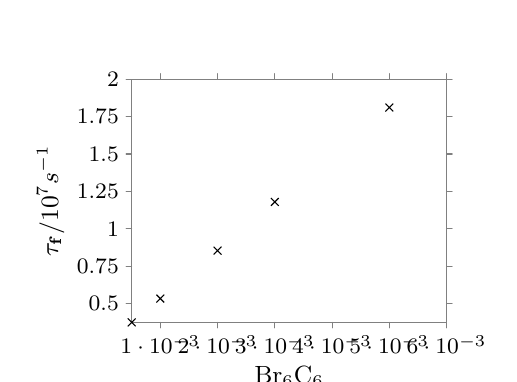
\begin{tikzpicture} 
\datavisualization [
	scientific axes, 
	visualize as scatter, 
	x axis = {length=4cm,include value=0.006, label={\ce{Br6C6}}}, 
	y axis={include value=2, label={\(\mathbf{\tau_f}/10^7s^{-1}\)}}
	]
data {
x, y
0.0005, 0.376
0.001,  0.535
0.002, 0.855
0.003, 1.18
0.005, 1.81
};
\end{tikzpicture}
\end{example}
\end{frame}

\begin{frame}
\begin{example}
We want to determine the values of \(k_f\) and \(k_q\) for pyrene\\\hspace{3pt}
The Stern-Volmer equation can be expressed in the form:
\[\frac{1}{\tau_f} = k_f + k_q[Q]\]
Therefore, plotting \ce{[Br6C6]} vs \(\tau^{-1}\) gives a straight line with\\ slope \(=k_q = 3.00\times10^9\ s^{-1}\) and\\ intercept \(=k_f = 1.98\times10^6\ s^{-1}\). 
\end{example}
\end{frame}

\begin{frame}
\frametitle{What you have learned to do in this lecture}
\begin{itemize}
\item Explain in words what the Franck-Condon Principle states
\item Explain why there is a mirror symmetry in absorption and fluorescence spectra
\item Solve simple problems involving rate coefficients and fluorescence lifetimes
\item Calculate fluorescence quantum yields in the presence of fluorescence quenchers
\item Derive the Stern-Volmer relationship
\end{itemize}
\end{frame}

\section{Polyatomic absorption}

\lecture{Polyatomic absorption}{Lecture 4}
\mode<presentation>{
	\begin{frame}
	\frametitle{Lecture outline}
		\begin{itemize}
		\item Some revision
		\item Chemical actonimetry example
		\item \(\sigma,\  \pi,\ n,\ \sigma^*\ and\ \pi^*\) electrons
		\item Polyatomic absorption
		\item Carbon-carbon double bonds
		\item Carbon-oxygen double bonds
		\end{itemize}
	\end{frame} }
	


\begin{frame}[shrink=20]{Mindmap example}
\resizebox{\textwidth}{!}{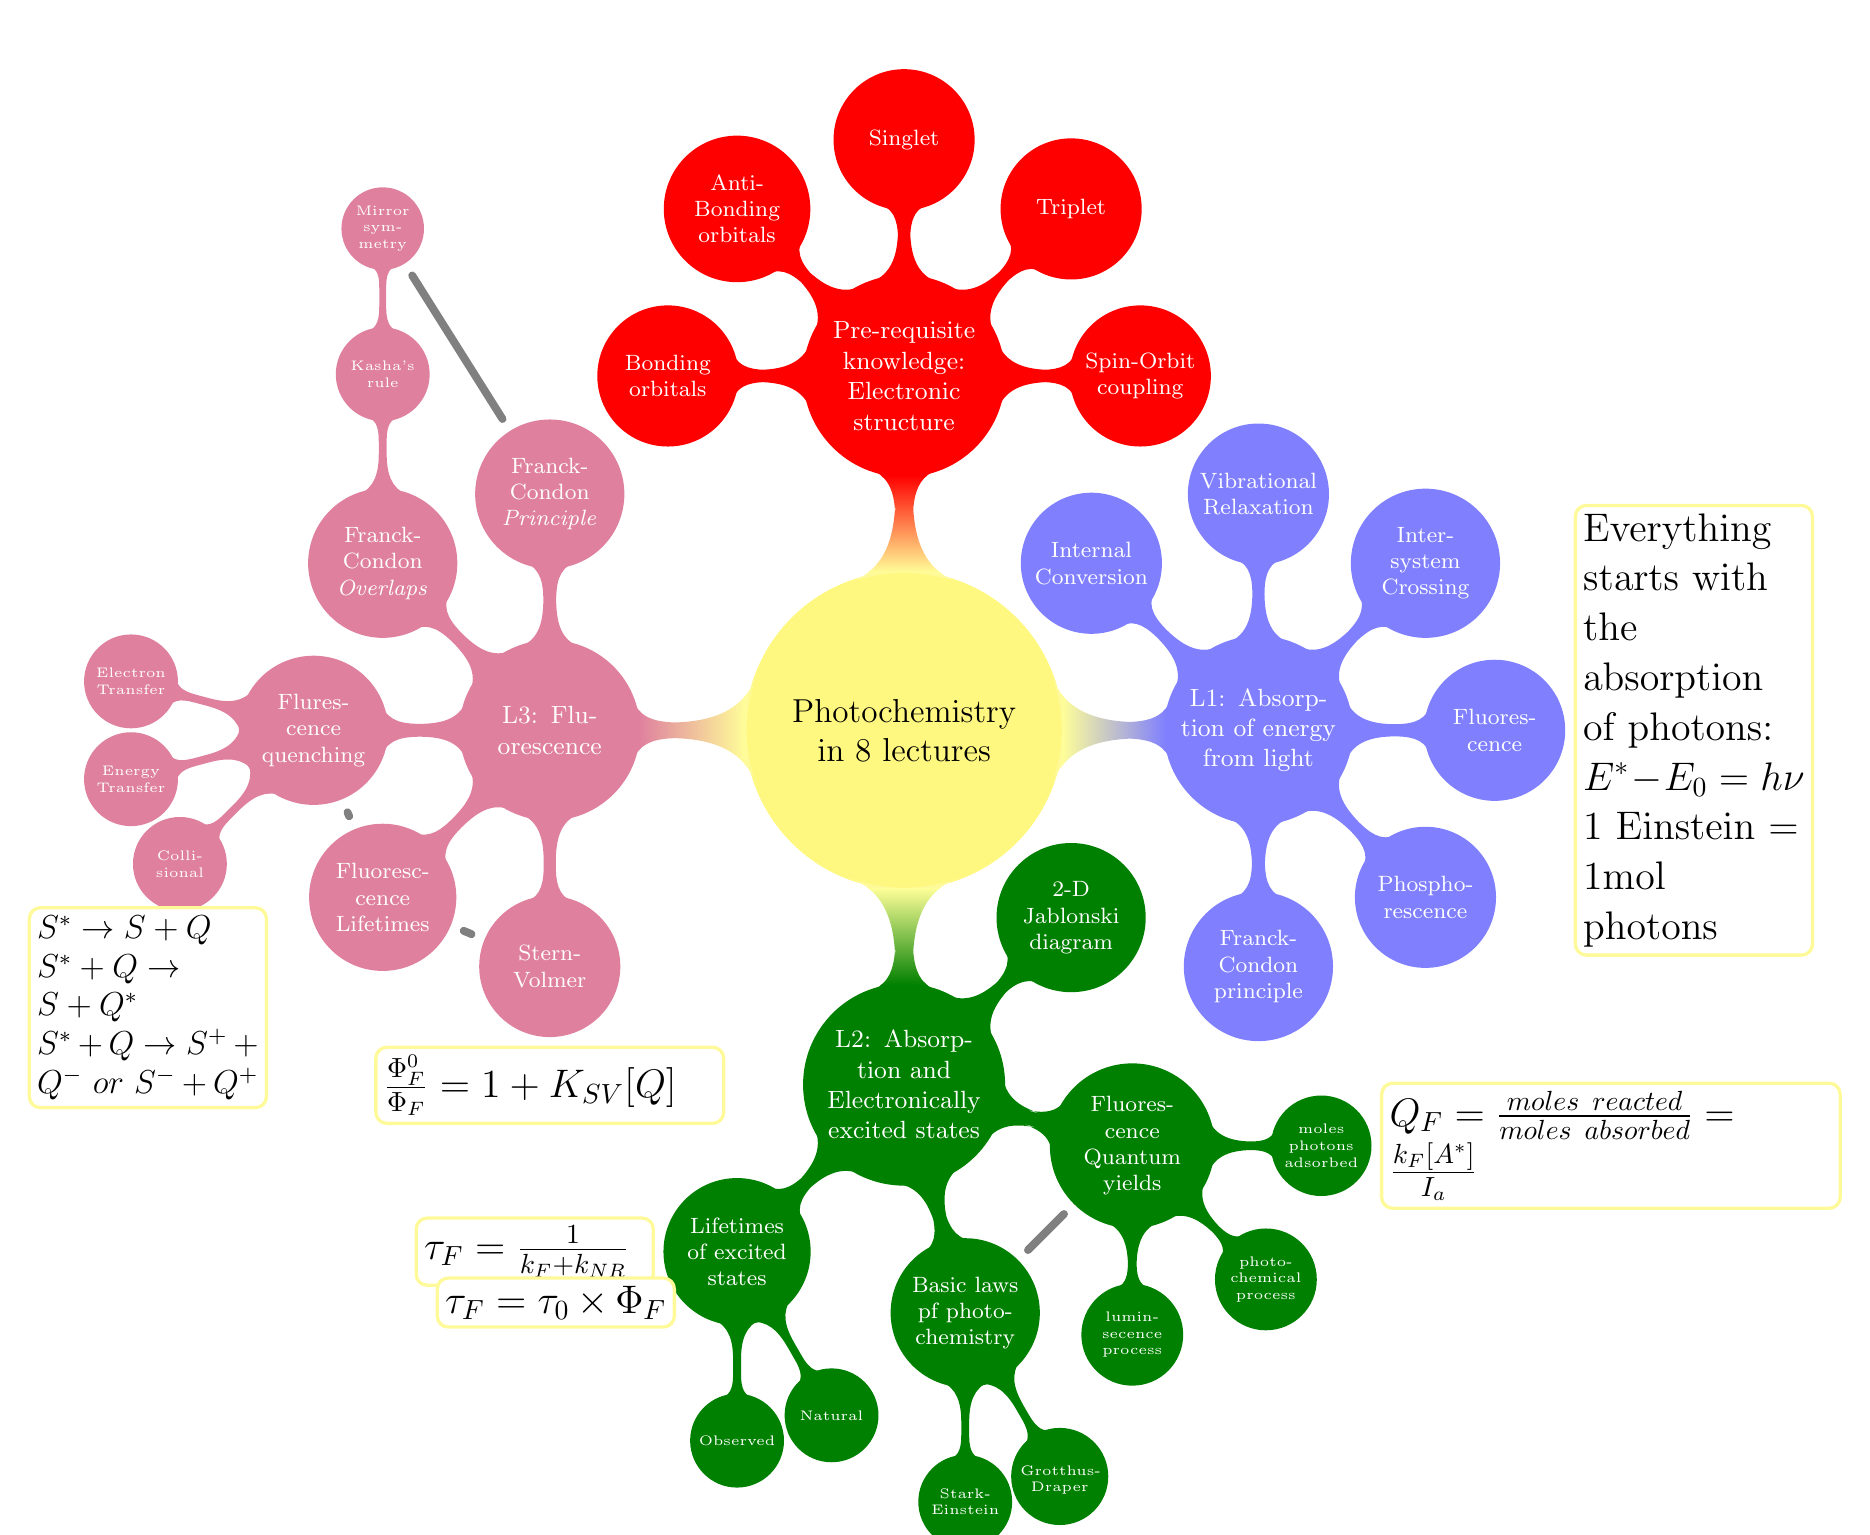
\begin{tikzpicture}
	[mindmap,
		every node/.style={concept, execute at begin node=\hskip0pt},
		concept color=yellow!40,text=white,
		grow cyclic,
		level 1/.append style={level distance=4.5cm,sibling angle=90},
		level 2/.append style={level distance=3cm}]
	\node[concept color=yellow!50,text=black] {Photochemistry in 8 lectures}
	[clockwise from=0,level 2 concept/.append style={sibling angle=45}]
	child[concept color=blue!50,visible on=<3->]{node[concept]{L1: Absorption of energy from light}[clockwise from=135]
			child{node[concept]{Internal Conversion}}
			child{node[concept]{Vibrational\\Relaxation}}
			child{node[concept]{Intersystem\\Crossing}}
			child{node[concept](fl){Fluorescence}}
			child{node[concept]{Phosphorescence}}
			child{node[concept]{Franck-Condon principle}}
	}
	child[concept color=green!50!black,visible on=<4->]{
		node[concept] (abs){L2: Absorption and Electronically excited states}
		[clockwise from=45,level 2 concept/.append style={sibling angle=60}]
		child{node[concept]{2-D Jablonski diagram}}
		child{node[concept](QF){Fluorescence Quantum yields}[clockwise from=0,level 3 concept/.append style={sibling angle=45}]
		child{node[concept](MA){moles photons adsorbed}
		}
		child{node[concept]{photochemical process}
		}
		child{node[concept]{luminsecence process}
		}
		}
		child{node[concept](laws){Basic laws pf photochemistry}[clockwise from=-60]
			child{node[concept]{Grotthus-Draper}}
			child{node[concept]{Stark-Einstein}}
		}
		child{node[concept](life){Lifetimes of excited states}[clockwise from=-60]
			child{node[concept]{Natural}}
			child{node[concept]{Observed}}
		}
	}
%	child[concept color=blue]{
%		node[concept]{Multiplicity}
%		[clockwise from=315]
%		child{node[concept]{Kasha's rule}}
%		child{node[concept]{Kasha's rule}}
%	}
	child[concept color = purple!50,visible on=<5->]{
		node[concept]{L3: Fluorescence}[counterclockwise from=90]
			child{node[concept](FCP){Franck-Condon \textit{Principle}}}
			child{node[concept](FCO){Franck-Condon \textit{Overlaps}}[clockwise from=90]
			child{node[concept](KR){Kasha's rule}[clockwise from=90]
				child{node[concept](MS){Mirror symmetry}}
			}
			}
			child{node[concept](FQ){Flurescence quenching}[clockwise from=225]
				child{node[concept](CQ){Collisional}}
				child{node[concept]{Energy Transfer}}
				child{node[concept]{Electron Transfer}}
			}
			child{node[concept](FL){Fluoresccence Lifetimes}}
			child{node[concept](SV){Stern-Volmer}}
	}
	child[concept color=red,visible on=<2->]{node[concept]{Pre-requisite knowledge: Electronic structure}
	[clockwise from=180]
		child{node[concept]{Bonding orbitals}}
		child{node[concept]{Anti-Bonding orbitals}}
		child{node[concept]{Singlet}}
		child{node[concept]{Triplet}}
		child{node[concept]{Spin-Orbit coupling}}
	}
	;
	\uncover<6>{
\begin{scope}[every annotation/.style={fill=white,text=black}]
	\node[annotation,right,text width = 8em,font=\Large] at (fl.east) {Everything starts with the absorption of photons:\\\(E^*-E_0=h\nu\)\\ 1 Einstein = 1mol photons};
	\node[annotation,right,text width=16em,font=\Large] at (MA.east){\(Q_F=\frac{moles\ reacted}{moles\ absorbed} = \frac{k_F[A^*]}{I_a} \)};
	\node[annotation,left,text width=8em,font=\Large] at (life.west) {\(\tau_F=\frac{1}{k_F + k_{NR}}\)};
	%\[ \Phi^\lambda = \frac{\textit{Rate of formation}}{I_a} \]
	\node[annotation,left,text width=8em,font=\Large] at (life.south west){\(\tau_F = \tau_0 \times \Phi_F\)};
	\node[annotation,below,text width=12em,font=\Large] at (SV.south){\( \frac{\Phi^0_F}{\Phi_F} = 1 + K_{SV}[Q] \)};
	\node[annotation,below,text width =8em,font=\large] at (CQ.south west){\(S^* \rightarrow S + Q\) \\ \(S^* + Q \rightarrow S + Q^*\) \\ \(S^* + Q \rightarrow S^+ + Q^-\ or\ S^- + Q^+\)};
\end{scope}
}
\uncover<6->{
	\draw [concept connection] (FCP) edge (MS);
	\draw[concept connection] (laws) edge (QF);
	\draw[concept connection] (FL) edge (FQ);
	\draw[concept connection] (SV) edge (FL);
	}
\end{tikzpicture}}
\end{frame}

\begin{frame}[label=actinometry]
\end{frame}

\begin{frame}[label=actinometry]
\frametitle{Chemical Actinometry}
\only<1>{
In chemical actinometry, the incident light is measured by monitoring a chemical reaction, like in the following example.
\begin{example}
The intensity of the incident light is measured by the decomposition of oxalic acid, \ce{(COOH)2} in the presence of uranyl sulfate (\ce{(UO2)SO4})

Light is absorbed leading to an excited state which causes decomposition of the oxalic acid:\\\hspace{5pt}

1) \ce{UO2+ + h$\nu$ -> (UO2+)^*}\\
2) \ce{(UO2+)^* + (COOH)2 -> UO2+ + H2O + CO2 + CO}\\\hspace{5pt}

For this reaction, \(\Phi = 0.53\), so we'll use quantum yield to determine the rate of incident photons.
\end{example}
}
\end{frame}
\begin{frame}[label=actinometry]
\frametitle{Chemical Actinometry}
\begin{example}
\only<1>{
Oxalic acid remaining after exposure for a fixed period of time, can be determined by titration with \ce{KMNO4}. The extent of decomposition of oxalic acid gives the number of incident photons.\\\hspace{5pt}

\ce{2MNO4- + 5H2C2O4 + 6H+ -> 2MN2+ + 10CO2 + 8H2O}\\\hspace{5pt}

A solution of 5.232 g oxalic acid in 25.0 ml water was irradiated for 300s. The remaining solution was titrated with 17.0 ml 0.212 M \ce{KMNO4 (aq)} for complete oxidation of remaining oxalic acid.
}
\only<2>{
Initial no. moles oxalic acid: \(\frac{5.232g}{90.03g/mol} = 0.058\ mol\)\\
Final no. moles oxalic acid: \(0.212\ mol/L\ \times 17\times 10^{-3}\ L\ \times ^5/_2 = 0.0901\ mol\)\\
Moles decomposed by light: 0.05811 - 0.00901 = 0.0491\\

\begin{multline*}\Phi = \frac{moles\ reacted}{moles\ absorbed} = 0.53 \implies\ moles absorbed = \frac{0.0491}{0.53}\\ = 0.093\ Einstein\end{multline*}

\begin{multline*}Rate\ of\ incidence\ =\frac{0.093\ Einstein}{300\ s} = 0.00031\ Einstein\ s^{-1}\\ = 1.86\times 10^{20} photons\ s^{-1}\end{multline*} 
}
\end{example}
\end{frame}

\begin{frame}
\frametitle{\(\sigma,\  \pi\),\ n, \(\sigma^*\) and \(\pi^*\) electrons}
\begin{description}
\item[\(\sigma\)-electrons] are localised between two atoms and are tightly bound\newline 
\(\Rightarrow\) Transitions from \(\sigma\)-orbitals are therefore quite \emph{high in energy} (typically vacuum-UV, \(\lambda\) = 100 -- 200 nm)
\item[\(\pi\) electrons] are more delocalised and bound less tightly than their \(\sigma\)-electrons.\newline
\(\Rightarrow\) Transitions from \(\pi\)-orbitals therefore occur at \emph{\underline{lower energy}} (typically far vacuum-UV,\(\lambda\) = 150 -- 250 nm for a single, unconjugated \(\pi\)-orbital)
\item[n electrons] are not involved in chemical bonding\newline
\(\Rightarrow\) Transitions from n-orbitals occur at the \emph{\underline{lowest energy}}, as the energy of a non-bonding orbital typically lies between that for bonding and anti-bonding orbitals
\(\Rightarrow\) n-orbitals are commonly \emph{\underline{O or N lone pairs}}, or non-bonding \(\pi\)-orbitals
\end{description}
\end{frame}

\begin{frame}
\begin{columns}[onlytextwidth]
\begin{column}{.5\textwidth}
\begin{figure}
\caption{\emph{\underline{valence electrons}} are shared in one or more bonds, and are the highest lying occupied states (HOMO)}
\includegraphics[width=\linewidth]{../graphics/energyvswave} 
\end{figure} 
\end{column}
\begin{column}{.5\textwidth}
\begin{figure}
\fbox{
\includegraphics[width=\linewidth]{../graphics/energyvsorbital}}
\caption{The energy required for an electron to transition to low lying unoccupied levels (LUMO) is characteristic of the \emph{\underline{bond}} from which it comes} 
\end{figure}
\end{column}
\end{columns}
\end{frame}

\begin{frame}
\frametitle{Polyatomic absorption}
\begin{columns}[onlytextwidth,T]
\begin{column}{.6\textwidth}
\begin{itemize}[<+->]
\item Any electron in a \emph{\underline{polyatomic molecule}} can be excited to an unoccupied level
\item We can \emph{\underline{separate electrons into various types}} that have characteristic spectral properties, \textit{i.e. n, \(\sigma\) and \(\pi\)} electrons
\item n-electrons are in a \emph{\underline{non-bonding}} ground state
\item \(\sigma\) and \(\pi\) electrons are in a stable \emph{\underline{bonding}} state
\item \(\sigma^*\) and \(\pi^*\) electrons are in an unstable \emph{\underline{anti-bonding}} state
\end{itemize}
\end{column}
\begin{column}{.4\textwidth}
\begin{figure}[h!]
\includegraphics[width=2in]{../graphics/orbitalenergies}
\caption{Generalised schematic diagram of orbital energies for large organic molecules}
\end{figure}
\end{column}
\end{columns}
\end{frame}

\begin{frame}[<+->]
\begin{itemize}
\item The {\color{red} chromophore} is a region in the molecule where the energy difference between two different molecular orbitals falls within the range of the visible spectrum
\item Visible light that hits the chromophore is absorbed by exciting an electron from its ground state into an excited state
\item The main chromophores that are encountered in organic photochemistry are {\color{red} carbon-carbon} and {\color{red} carbon-oxygen} double bonds
\item[]<1-> \includegraphics[width=\linewidth]{../graphics/pi2pistar}
\end{itemize}
\end{frame}

\subsection{C=C and C=O}

\begin{frame}
\frametitle{carbon-carbon double bounds}
\onslide*<1>{
\begin{itemize}
\item Consider \emph{ethene} as a model compound
\item The carbons in ethene are \emph{\underline{\(sp^2\)-hybridized}}
\end{itemize}
\begin{figure}[t]
\includegraphics[width=.3\textwidth]{../graphics/ethene}
\end{figure}
The ground state electronic configuration of carbon is \(1s^22s^22p^2\)
\begin{figure}[h]
\centering
\includegraphics[width=.7\textwidth]{../graphics/groundstateelectrons}
\end{figure} }
\onslide*<2>{
\begin{figure}[h]
\includegraphics[width=.3\textwidth]{../graphics/sp2}
\end{figure}
\textbullet Three \(sp^2\) hybrid orbitals are formed and these arrange themselves as far apart in space as they can -- at 120\(\circ\) to each other\newline
\textbullet The remaining p orbital is at right angles to them}
\onslide*<3>{
\begin{figure}[h]
\centering
\includegraphics[width=\textwidth]{../graphics/hybridizedorbitals}
\caption{The two carbon atoms and four hydrogen atoms would look like this before they join together}
\end{figure} }
\onslide*<4> {
\begin{figure}[h]
\includegraphics[width=\textwidth]{../graphics/sigmapiorbitals} 
\end{figure} }
\onslide*<5>{
\begin{figure}[t]
\includegraphics[width=.5\textwidth]{../graphics/bondantibond}
\end{figure}
The sideways overlap of two p-orbitals leads to a \(\pi\) bonding molecular orbital and a \(\pi^*\) anti-bonding molecular orbital\newline
\fcolorbox{black}{yellow}{\textcolor{black}{\parbox{.9\textwidth}{The \(\pi\) and \(\pi^*\) orbitals have a \emph{\underline{strong overlap}}\newline
Therefore, the \(\pi\) to \(\pi^*\) transition has a \emph{\underline{high probability}} of taking place}}} }
\onslide*<6> {
\begin{columns}[onlytextwidth]
\begin{column}{.4\textwidth}
\begin{figure}[t]
\includegraphics[width=\columnwidth]{../graphics/etheneorbitals}
\caption{The two highest occupied and two lowest unoccupied molecular orbitals of ethene}
\end{figure}
\end{column}
\begin{column}{.6\textwidth}
\begin{itemize}
\item As shown earlier, ethene has 5 \(\sigma\)-orbitals and 1 \(\pi\) orbital
\item The \(\pi_1\) orbital corresponds to the plus (\emph{\underline{symmetric}}) combinations of \(\pi\)-orbitals
\item The \(\pi_2^*\) orbital corresponds to the minus (\emph{\underline{antisymmetric}}) combinations of \(\pi\) orbitals
\end{itemize}
\end{column}
\end{columns} 
}
\end{frame}

\begin{frame}
\frametitle{carbon-oxygen double bonds}
\onslide*<1>{
\begin{columns}[onlytextwidth]
\begin{column}{.5\textwidth}
\begin{itemize}
\item Consider \textbf{\underline{methanal}} as a model compound
\item The carbon and oxygen atoms in methanal are \(sp^2\)-\emph{\underline{hybridized}}
\end{itemize}
\end{column}
\begin{column}{.5\textwidth}
\includegraphics[width=\columnwidth]{../graphics/methanal}
\end{column}
\end{columns}
\begin{itemize}
\item The ground state electronic configuration of oxygen is \(1s^22s^22p^4\)
\item[] \includegraphics[width=0.8\textwidth]{../graphics/methanalelectronconfig}
\end{itemize}
}
\onslide*<2>{
\centering
Two of the \(sp^2\) hybrid orbitals contain lone pairs of electrons \vspace{10pt}
\bigskip
\includegraphics[width=0.5\textwidth]{../graphics/methanal2}
}
\onslide*<3>{
\centering
\includegraphics[width=.8\textwidth]{../graphics/carboxbond}
\begin{itemize}
\item The \emph{\underline{distribution of electrons}} in the \(\pi\)-bond is heavily distorted towards the oxygen end of the bond, because oxygen is much more \emph{\underline{electronegative}} than carbon
\item This causes \emph{\underline{major differences in the reactions of compounds}} containing carbon-oxygen double compared with compounds containing carbon-carbon double bonds
\end{itemize}
}
\onslide*<4>{
\centering
\begin{figure}[h!]
\includegraphics[width=.5\textwidth]{../graphics/methanal3}
\caption{Methanal has \(3\sigma\), \(1\pi\) and 2 \textit{n} orbitals}
\end{figure}
\fcolorbox{black}{yellow}{\textcolor{black}{\parbox{.7\textwidth}{The \textit{n} and \(\pi^*\) orbitals have \emph{\underline{no overlap}}, they are essentially orthogonal}}}
}
\onslide*<5>{
\centering
\begin{figure}[h!]
\includegraphics[width=.5\textwidth]{../graphics/methanaldiagram}
\caption{The four highest occupied and two lowest unoccupied molecular orbitals of methanal}
\end{figure}
\medskip
\textbullet Therefore, the \textit{n} to \(\pi^*\) transition has a \emph{\underline{low probability}} of taking place
}
\end{frame}

\subsection{Absorption efficiency}

\begin{frame}[label=molabs]
\frametitle{Molar absorption coefficients}
\begin{table}[h!]
\caption{Molar absorption coefficient values usually found for different types of tranisition}
\begin{tabular}{c c}
	\textbf{Transition type} & \textbf{\(\epsilon/L mol^{-1}cm^{-1}\)}\\\hline
	\(\pi \rightarrow \pi^*\) & 5,000 - 200,000\\
	\(n \rightarrow \sigma^*\) & 100 - 1,000\\
	\(n \rightarrow \pi^*\) & 1-400\\\hline
\end{tabular}
\end{table}
\textbullet \(\epsilon_{max}\) is an indicator of the \emph{\underline{probability}} of a transition\newline\bigskip
\textbullet Weaker (less probable) transition \(\implies\) smaller value of \(\epsilon_{max}\)
\hyperlink{spontaneous<7>}{\beamerreturnbutton{spontaneous emission}}
\end{frame}

\begin{frame}
\frametitle{Absorption maxima}
\begin{table}[h!]
\caption{The absorption maxima (\(\lambda_{max}\)) are variable due to the varying electronegativity of the heteroatoms}
\begin{tabular}{c c}
\textbf{Compound} 		&	\textbf{\(\lambda_{max}\)/ nm}\\\hline\rule{0pt}{1.2em}
CH\(_2\)=CH\(_2\)		&	173\\
(CH\(_3\))CH=CH\(_2\)	&	173\\
\textit{cis}-(CH\(_3\))CH=CH(CH\(_3\))	&	175\\
\textit{trans}-(CH\(_3\))=CH(CH\(_3\))	&	178\\
CH\(_2\)=CH(Cl)	&	183\\
\textit{cis}-(Cl)CH=CH(Cl)	&	193\\
\textit{trans}-(Cl)CH=CH(Cl)	&	200\\
\textit{trans}-(Br)CH=CH(Br)	&	210\\
Cl\(_2\)=Cl\(_2\)	&	205\\\hline
\end{tabular}
\end{table}
\end{frame}

\begin{frame}
\frametitle{Solvatochromic shifts}
\only<1>{
The effects of solvents on the absorption maxima (\(\lambda_{max}\)) of the \(n \rightarrow \pi^*\) transitions in acetone, (CH\(_3\)CO(CH\(_3\))
\begin{columns}[onlytextwidth]
\begin{column}{.5\textwidth}
\begin{tabular}{c c}
\textbf{Solvent} 	& \(\lambda_{max}\) /nm\\\hline
Vapour	&	277\\
Hexane	& 279\\
Chloroform	&	277\\
Ethanol	&	272\\
Methanol	&	270\\
Water	& 264\\\hline
\end{tabular}
\end{column}
\begin{column}{.5\textwidth}
\begin{itemize}
\item When reporting the absorption maxima of carbonyl compounds the \emph{\underline{solvent}} is given for the data as the position of the \(n \rightarrow \pi^*\) transitions can vary as musch as 15 nm in different solvents
\item Such changes in the spectrum with solvent are called \emph{\underline{solvatochromic shifts}}
\end{itemize}
\end{column}
\end{columns}
}\only<2>{
\textbullet In \emph{\underline{non-polar solvents}}, the dipolar interactions are negligible both in the ground and the excited state\break\bigskip
\textbullet In \emph{\underline{water}}, the strength of dipolar interactions is significant\newline
\url{http://people.chem.ucsb.edu/kahn/kalju/chem126/public/solvat_intro.html}
}
\end{frame}

\begin{frame}
\frametitle{Solvatochromic shifts}
\begin{itemize}
\item The nature and \emph{relative energies of the electronic states} of a molecule determine its photophysical and photochemical properties
\item The \emph{environment} in which a molecule is immersed can alter these states
\item This in turn \emph{modifies the properties}, giving rise, for instance, to solvatochromic shifts in absorption and emission UV/Vis spectra
\end{itemize}
\end{frame}

\begin{frame}
\begin{figure}
\begin{overpic}[width=.8\textwidth]{../graphics/solvatochromic}
\put(65,25){\includegraphics[width=.3\textwidth]{../graphics/nilered}}
\end{overpic}
\caption{Calculated absorption spectra for nile red (Zuehlsdorff \textit{et al.}, JCP 146 (\textbf{2017})}
\end{figure}
\end{frame}

%\begin{frame}
%\begin{figure}
%\includegraphics[width=.6\textwidth]{../graphics/valence}\break
%\caption{\underline{Valence electrons} are shared in one or more bonds, and are the highest lying occupied states (HOMO)}
%\end{figure}
%\end{frame}
%
%\begin{frame}
%\begin{figure}
%\includegraphics[width=.5\textwidth]{../graphics/energywavelength}
%\caption{The energy required for an electron to transition to low lying unoccupied levels (LUMO) is characteristic of the \underline{bond} from which it comes}
%\end{figure}
%\end{frame}



%\begin{frame}
%\LARGE{Directed study}
%\begin{itemize}
%\item The selection rules for electronic transitions
%\item Quantum numbers
%\begin{itemize}
%\item The principal quantum number, \textsl{n}
%\item Theorbital angular momentum quantum number, \textsl{l}
%\item The magnetic quantum number, \(m_l\)
%\item The electron spin quantum number, \(m_s\)
%\item Coupling of angular momentum (spin, orbital)
%\end{itemize}
%\item Total spin quantum number, S
%\item Multiplicity
%\end{itemize}
%\end{frame}

\begin{frame}
\frametitle{What you should know after this lecture}
\begin{itemize}
\item The difference between \(\sigma,\  \pi\),\ n, \(\sigma^*\) and \(\pi^*\) electrons
\item Describe different types of electronic transition and their probabilities
\item Explain the relationship between molar attenuation coefficient and electronic transition types
\item Explain how electronegativity affects the position (wavelength) of the absorption maximum
\item Explain the effect of solvent on electronic transition (absorption maximum)
\end{itemize}
\end{frame}

\lecture{Adsorption to emission 2: Phosphorescence, intersystem crossing and the triplet state}{Lecture 5}
\begin{frame}
	\frametitle{Lecture contents}
		\begin{itemize}
			\item Example problem, fluorescence quenching
			\item Phosphorescence
			\item Singlet-Triplet splitting
			\item The energy gap law
			\item Triplet states
		\end{itemize}
	\end{frame}

\begin{frame}
\frametitle{Example problem -- fluorescence quenching and Stern-Volmer}
\begin{example}
\only<1>{
Benzophenone + \(h\nu \rightarrow S_1^* \rightarrow T_1^* \rightarrow \) Phosphorescence \(\rightarrow S_0 + h\nu\)

\medskip The reaction takes place in a solvent (methanol) and there is a quencher, Q, present (Triethylamine)

\medskip The half-life, \(t_{1/2}\), of the fluorescence without quencher is 29 \(\mu s\)

\medskip What is the value of \(k_q\)?}

\only<2>{To solve the problem, summarise what we know:

\medskip\begin{tabular}{cc}
[Q] / (mol L\(^{-1}\)) & I\(_f\) \\\hline
0.0010 & 0.41\\
0.0050& 0.25\\
0.0100 & 0.16\\\hline
\end{tabular}
Half-life = \(t_{1/2}= 29 \mu s\)

\medskip Remember, half-life, \(t_{1/2}\) is NOT the same as the lifetime, \(\tau_f\), but \(\tau_f = \frac{ln2}{t_{1/2}}\) (why? because \(I_f\) decays as \(e^{-k_ft} = e^{-t/\tau_f}\) in the absence of quencher)
}
\only<3>{
The processes are: 

\smallskip
\begin{tabular}{lcl}
Process & Rate coefficient & Rate\\\hline
Absorption & \(k_a\) & \( k_a[S_1^*] = I_a\)\\
Fluorescence & \(k_f\) & \(k_f[S_1^*]\)\\
ISC & \(k_{ISC}\) & \(k_{ISC}[S_1^*]\)\\
Quenching & \(k_q\) & \(k_q[S_1^*][Q]\)\\\hline
\end{tabular}

The emission has been measured under constant irradiation, so measurements are made during steady state process:

\smallskip Production of excited singlet state, \(S_1^*\) = Losses of \(S_1^*\)
}
\only<4>{
\smallskip \begin{multline*}\frac{d[S_1^*]}{dt} = k_a[S_1^*] - k_f[S_1^*] - k_q[S_1^*]\\
= I_a - k_f[S_1^*] - k_q[S_1^*] = 0\end{multline*}

That means

\([S_1^*] = \frac{I_a}{k_f + k_q[Q]}\), and \(I_f = k_f[S_1^*] = \frac{k_q[Q]}{k_fI_a}\)


So if we measure \(I_f\) at different concentrations of Q, we can plot 1/\(I_f\) vs. [Q]
}
\end{example}
\end{frame}
%\only<5>{
\begin{frame}[fragile]
\begin{example}
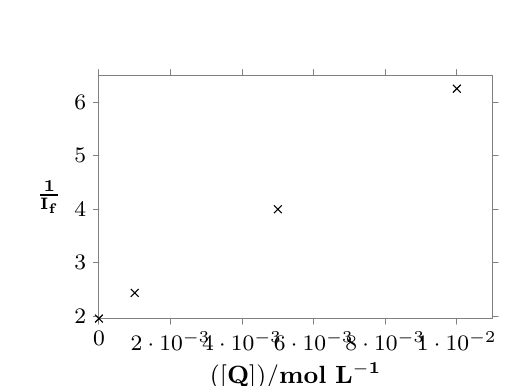
\begin{tikzpicture} 
\datavisualization [
	scientific axes={upright labels}, 
	visualize as scatter, 
	x axis = {include value=0.011, label={{\(\mathbf{([Q])/mol\ L^{-1}}\)}}}, 
	y axis={include value=6.5, label={\(\mathbf{\frac{1}{I_f}}\)}}
	]
data {
x, y
0, 1.96
0.0010, 2.439
0.0050, 4
0.0100, 6.25
};
\end{tikzpicture}Fit line

Intercept = \(\frac{1}{I_a} = 1.96 \implies I_a=0.51\)

Slope = \(\frac{k_q}{k_fI_a} = 424.5 \implies k_q=0.51\times 424.5\times k_f\)

\medskip But what is \(k_f\)?
\end{example}
\end{frame}

\begin{frame}
\begin{example}
Remember \(\tau_f = \frac{ln2}{t_{1/2}}\), so \(k_f = \frac{ln2}{t_{1/2}}\)

\bigskip \begin{multline*}\implies k_q = 0.51 \times 424.5\ L\ mol^{-1} \times \frac{ln2}{29\times 10^{-6}\ s}\\=5.17\times 10^6\ L\ mol^{-1}s^{-1}\end{multline*}
\end{example}
\end{frame}

\section{Phosphorescence, intersystem crossing and the triplet state}
\begin{frame}
\frametitle{Phosphorescence, ISC and the Triplet state}
\textbf{Phosphorescence} (pink arrow) is an \underline{emissive pathway} between two levels of \underline{different multiplicity} (\(\Delta S \neq 0\)) and \underline{different energy}, e.g. \(T_1 \rightarrow S_0\) in organic molecules.\\
\includegraphics[width = .5\textwidth]{../graphics/phosphor}\\
The triplet state is populated almost exclusively via \underline{intersystem crossing} from the first excited singlet state  (\(S_1 \rightsquigarrow T_n \rightsquigarrow T_1\))
\end{frame}

\begin{frame}
\frametitle{Phosphorescence}
\begin{columns}[onlytextwidth]
\begin{column}{.5\textwidth}
The ``forbidden'' nature of the luminescence leads to the ``long'' lifetimes measured (milliseconds to seconds)

In its most simple consideration the \underline{triplet state} can be regarded as a molecule with two parallell unpaired electron spins, i.e. a \underline{paramagnetic species}

\end{column}
\begin{column}{.5\textwidth}

\includegraphics[height=\textwidth]{../graphics/spinforbidden}

\end{column}
\end{columns}
\end{frame}

\begin{frame}
\frametitle{Spin-orbit coupling}
\begin{columns}[onlytextwidth]
\begin{column}{.5\textwidth}
\textbf{Spin-Orbit coupling} makes the forbidden transition T \(\rightarrow\) S (weakly) allowed.

Since the transition is only weakly allowed, the process is not very effective.

The process happens in atoms that have strong spin-orbit coupling and is more effective for substances where the energy transfer is less effective

\end{column}
\begin{column}{.5\textwidth}

\includegraphics[height=\textwidth]{../graphics/phosphor2}
\end{column}
\end{columns}
\end{frame}

\subsection{Origin of Singlet-Triplet (S-T) splitting}
\begin{frame}
\begin{itemize}
\item The triplet of any particular state (T\textsubscript{1}, T\textsubscript{2}, ..., T\textsubscript{n}) is always of \textit{\underline{lower energy}} than the corresponding singlet (S\textsubscript{1}, S\textsubscript{2}, ..., S\textsubscript{n})
\item The origin of this is purely \textit{\underline{electrostatic}} in nature
\item Singlet and triplet states have different energies because the electrons in these states have \textit{\underline{different spatial distributions}}: 	
\end{itemize}
\end{frame}

\begin{frame}
\frametitle{Fluorescence-Phosphorescence}

\includegraphics[width=.5\textwidth]{../graphics/naphtalenejab}\\

\end{frame}

\begin{frame}
\frametitle{Timescales for fluorescence and phosphorescence}

\includegraphics[width=.5\textwidth]{../graphics/timescales}
\end{frame}

%\begin{frame}
%\frametitle{Molecular oxygen as a ``Triplet excited state quencher''}
%\begin{columns}[onlytextwidth]
%\begin{column}{.5\textwidth}
%Molecular O\textsubscript{2} is unusual in that it exists as a \underline{triplet in the ground state}
%
%O\textsubscript{2} can therefore quench the triplet excited state of species
%
%This leads to a decrease in the quantum yield of phosphorescence (\(\Phi_p\))
%\end{column}
%\begin{column}{.5\textwidth}
%\includegraphics[width=7\TPHorizModule]{../graphics/oxygen}
%\end{column}
%\end{columns}
%\end{frame}

\subsection{Intersystem Crossing}

\begin{frame}
\frametitle{Intersystem Crossing}
\begin{itemize}
\item \textbf{Intersystem crossing} (ISC) is the \emph{non-radiative} transition of an electron between two states of different \underline{multiplicity} (\(\Delta S \neq 0\)) \includegraphics[width=.25\textwidth]{../graphics/intersystem}
\item It is the energy gap between S and T which controls the efficiency of intersystem crossing
\item Large gap -- small \(k_{ISC}\) and vice versa
\item If the gap is large, there will be a great difference in charge densities \(\implies\) can expect a large reactivity difference between S and T
\item If the gap is small, the difference in charge distribution for S and T will be small \(\implies\) can expect similar singlet-triplet chemical reactivities
\end{itemize}
\end{frame}

The singlet and triplet excited states share a common geometry at the point where their potential energy curves intersect. If there is a mechanism for unpairing two electron spins (and acheiving the conversion of \ce{ ^ v} to \ce{ ^ ^}), the molecule may undergo \textbf{intersystem crossing} and become a tripelt state. If an excited molecule crosses into a triplet state, it continues to deposit energy into the surroundings. But it is now stepping down the triplet's vibrational ladder, and at the lowest energy level it is trapped because the triplet state is at a lower energy than the corresponding singlet (remember Hund's rule from CM3016). The solvent cannot absorb the final, large quantum of electronic excitation energy and the molecule cannot radiate its energy because return to the ground state is spin-forbidden.

The radiative transition, however, is not totally forbidden because the spin-orbit coupling that that was responsible for the intersystem crossing also breaks the selection rule. The molecules are therefore able to emit weakly, and the emission may continue long after the original excited state was formed.

This mechanism also suggests that phosphorescence should be most intense from solid samples, because energy transfer is then less efficient and intersystem crossing has time to occur as the singlet excited state steps slowly past the intersection point.

The mechanism also suggests that the phosphorescence efficiency should depend on the presence of a moderately heavy atom (with strong spin-orbit coupling).

\begin{frame}
\frametitle{Why does the S-T splitting decrease as the size of the molecule increases?}
In a \underline{large molecule} the electrons are spread out over more space (larger box!)\\
\hspace{5pt} \(\implies\) Less Coulombic repulsion (electrostatic interactions) between the electrons\\
\hspace{10pt} \(\implies\) More stable \\
\hspace{15pt} \(\implies\) Less S-T splitting\\
\medskip

In a \underline{small molecule} the electrons are confined to a smaller space (smaller box!)\\
\hspace{5pt} \(\implies\) More Coulombic repulsion (electrostatic interactions) between the electrons\\
\hspace{10pt} \(\implies\) Less stable\\
\hspace{15pt} \(\implies\) More S-T splitting
\end{frame}

\begin{frame}
\frametitle{Why is S-T splitting larger for \(\pi^* \leftarrow \pi\) excitations than \(\pi^* \leftarrow n\) excitations?}
\begin{columns}[onlytextwidth]
\begin{column}{.5\textwidth}
\includegraphics[width = 6\TPHorizModule]{../graphics/excitations}
\end{column}
\begin{column}{.5\textwidth}
\begin{itemize}
\item The \(\pi\) and \(\pi^*\) orbitals have a \underline{strong overlap}
\item The \(\pi\) and \(\pi^*\) orbitals are therefore in the \underline{same region of space}
\item \hspace{5pt} More Coulombic repulsion between the electrons, making it less stable and giving more S-T splitting
\end{itemize}
\end{column}
\end{columns}
\end{frame}

\begin{frame}
\frametitle{Why is S-T splitting larger for \(\pi^* \leftarrow \pi\) excitations than \(\pi^* \leftarrow n\) excitations?}
\begin{columns}[onlytextwidth]
\begin{column}{.5\textwidth}
\includegraphics[width = 6\TPHorizModule]{../graphics/methanal3}
\end{column}
\begin{column}{.5\textwidth}
\begin{itemize}
\item The n and \(\pi^*\) orbitals have \underline{no overlap}, they are essentially orthogonal
\item The n and \(\pi^*\) orbitals are therefore \underline{not in the same region of space}
\item \hspace{5pt} Less Coulombic repulsion between the electrons, making it more stable and giving less S-T splitting
\end{itemize}
\end{column}
\end{columns}
\end{frame}

\begin{frame}
\frametitle{The energy gap law}
This means that S\textsubscript{1} to T\textsubscript{1} intersystem crossing (ISC) will be highly probable in ketones but improbable in alkenes\newline\smallskip
\begin{columns}[onlytextwidth]
\begin{column}{6\TPHorizModule}
\fbox{\parbox{\textwidth}{ \centering \textbf{ALKENES} \hfill \\
Large overlap of orbitals (\(\pi^* \leftarrow \pi\)) in the same region of space\\
\(\implies\) Large Coulombic repulsion between the electrons\\
\(\implies\) Less stable\\
\(\implies\) More S-T splitting\\
\(\implies\) \underline{ISC inefficient} }}
\end{column}
\begin{column}{6\TPHorizModule}
\fbox{\parbox{\textwidth}{ \centering \textbf{KETONES} \hfill \\
Little overlap of orbitals (\(\pi^* \leftarrow n\)) in the same region of space\\
\(\implies\) Less Coulombic repulsion between the electrons\\
\(\implies\) More stable\\
\(\implies\) Less S-T splitting\\
\(\implies\) \underline{ISC efficient} }}
\end{column}
\end{columns}
\end{frame}

\begin{frame}
\frametitle{Electronic transitions, configurations and states}
\includegraphics[width=\textwidth]{../graphics/electronictransitions}
\end{frame}

\begin{frame}
\begin{tabular}{lcll}
Compound & Structure & \(\Delta E(S_1 - T_1)/cm^{-1}\) & S-T splitting\\\hline
Benzene & \includegraphics[height=1cm]{../graphics/benzene} & 8,800 & Large\\
Naphtalene & \includegraphics[height=1cm]{../graphics/naphtalene} & 10,800 & Large\\
Anthracene & \includegraphics[height=1cm]{../graphics/anthracene} & 11,500 & Large\\
Ethylene/Ethene & \includegraphics[height=1cm]{../graphics/ethylene} & 24,000 & Large\\
Acetone & \includegraphics[height=1cm]{../graphics/acetone} & 3,000 & Smaller\\
Acetophenone & \includegraphics[height=1cm]{../graphics/acetophenone} & 1,820 & Smaller\\
Benzophenone & \includegraphics[height=1cm]{../graphics/benzophenone} & 2,200 & Smaller\\\hline
\end{tabular}
\end{frame}

\begin{frame}
\frametitle{Why does the energy gap control the rate of intersystem crossing?}
\begin{columns}[onlytextwidth]
\begin{column}{6\TPHorizModule}
\fbox{\parbox{\textwidth}{\hfill \textbf{Large S-T splitting}, e.g. alkenes \hfill \\
The triplet (T) state is pure, it has very little singlet character (S)\\
\(\implies\) Little or no \underline{singlet/triplet mixing}\\
\(\implies\) Emission transition to the ground state singlet forbidden\\
\(\implies\) Leads to a \underline{long-lived triplet} state (seconds)
}}
\end{column}
\begin{column}{6\TPHorizModule}
\fbox{\parbox{\textwidth}{\hfill \textbf{Small S-T splitting}, e.g. ketones \hfill \\
The triplet (T) state is not very pure, it has some singlet character (S)\\
\(\implies\) This is known as \underline{singlet/triplet mixing}\\
\(\implies\) Emission transition to the ground state less forbidden\\
\(\implies\) Leads to a \underline{short-lived triplet} state (milliseconds)\\
}}
\end{column}
\end{columns}
\end{frame}

\subsection{Properties of Triplet states}

\begin{frame}
\frametitle{Properties of triplet states}
Molecules may \underline{phosphoresce} in competition with \emph{radiationless deactivation} to ground state, or react or participate in \underline{triplet energy transfer} (i.e. pass triplet energy to triplet of an acceptor molecule)\newline\medskip

It is generally observed:\newline
\begin{itemize}
\item \(\pi \rightarrow \pi^*\) states phosphoresce strongly in solid, never in gas
\item \(n \rightarrow \pi^*\) states may phosphoresce in both phases
\item \(\pi \rightarrow \pi^*\) states have intrinsic \(\tau_T\) lifetimes in order of \underline{seconds}
\item \(n \rightarrow \pi^*\) states have intrinsic \(\tau_T\) lifetimes in order of \underline{milliseconds}
\end{itemize}
\end{frame}

\begin{frame}
\frametitle{Molecular oxygen as a ``Triplet excited state quencher''}
\begin{columns}[onlytextwidth]
\begin{column}{.5\textwidth}

Molecular O\textsubscript{2} is unusual in that it exists as a \underline{triplet in the ground state}

O\textsubscript{2} can therefore quench the triplet excited state of species

This leads to a decrease in the quantum yield of phosphorescence (\(\Phi_p\))

\end{column}
\begin{column}{.5\textwidth}

\includegraphics[width=7\TPHorizModule]{../graphics/oxygen}
\end{column}
\end{columns}
\end{frame}
	
\begin{frame}
\frametitle{Why do \(\pi \rightarrow \pi^*\) states phosphoresce strongly in solid, never in gas wehereas n\(\pi^*\) states may phosphoresce in both phases?}
A: States that last for a long time are much more likely to be \underline{quenched} by a bimolecular collision

\only<1>{\fbox{\parbox{\textwidth}{ \(\mathbf{\pi \pi^*}\) states  \\
Intrinsic \(\tau_T\) lifetimes in order of \underline{seconds}\\
\(\implies\) In the gas phase the likelihood of the triplet being quenched by a bimolecular collision is very high\\
\(\implies\) No phosphorescence, \underline{fluorescence more important}\\
\(\implies\) In the solid phase the likelihood of the triplet being quenched by a bimolecular collision is much lower\\
Strong phosphorescence
}}}
\only<2>{
\fbox{\parbox{\textwidth}{n\(\mathbf{\pi^*}\) states \\
Intrinsic \(\tau_T\) lifetimes in order of \underline{milliseconds}\\
\(\implies\) Triplet state less easily quenched due to an order of magnitude difference in the lifetime\\
\(\implies\) Phosphorescence and intersystem crossing important\\
}}}
\end{frame}

\begin{frame}
\frametitle{Why do compounds in which the lowest excited singlet state is n\(\pi^*\) in nature not usually fluoresce strongly?}
\begin{itemize}[<+->]
\item \emph{Little overlap of orbitals} (\(n \rightarrow \pi^*\)) in the same region of space
\item Less orbital overlap leads to \emph{less coulombic repulsion}
\item Less coulombic repulsion causes \emph{less singlet-triplet (S-T) splitting}
\item More singlet/triplet mixing means that:\\
\hspace{10pt} \(S_1 \rightarrow T_n\) intersystem crossing is efficient (\(k_{ISC}\) is large)\\
\hspace{10pt} \(S_1 \rightarrow S_0\) internal conversion is comparatively inefficient (\(k_{IC}\) is small)
\item Thus, the singlet state becomes depopulated and the triplet state populated
\item This leads to an \emph{increase} in \(\tau_0\) as S \(\rightarrow\) T processes are spin forbidden
\item Since \(\tau_0 = \frac{1}{k_F}\), as \(\tau_0\) increases, the rate of fluorescence decreases
\end{itemize}
\end{frame}

\begin{frame}
\frametitle{Summary: properties of triplet states in ALKENES}
% Define block styles
\tikzstyle{block} = [rectangle, draw, fill=blue!20,  align=left,
   text centered, rounded corners, minimum height=4em]
\tikzstyle{line} = [draw, -latex']
    
\begin{tikzpicture}[node distance = 3cm, auto,font=\footnotesize]
    % Place nodes
    \node [block] (1st) {Orbitals (\(\pi \rightarrow \pi^*\))\\ in the same\\ region of space,\\ large overlap};
\uncover<2->{    \node [block, right of=1st,node distance = 3.5cm] (2nd) {Large Coulombic\\ repulsion between\\ the electrons};     \path [line] (1st) -- (2nd);}
\uncover<3->{    \node [block, right of=2nd] (3rd) {Less \\stable}; \path [line] (2nd) -- (3rd);}
\uncover<4->{    \node [block, right of=3rd,node distance=2cm] (4th) {Large S-T\\ splitting}; \path [line] (3rd) -- (4th);}
\uncover<5->{    \node [block, below of=4th,node distance=2.2cm] (5th) {The triplet\\ state is pure,\\ no S/T mixing}; \path [line] (4th) -- (5th);}
\uncover<6->{    \node [block, left of=5th,node distance=2.5cm] (6th) {ISC inefficient};  \path [line] (5th) -- (6th);}
\uncover<7->{    \node [block, left of=6th,node distance=3.5cm] (7th) {Emission transition\\ to the ground\\ state\\ singlet strongly\\ forbidden}; \path [line] (6th) -- (7th);}
\uncover<8->{    \node [block, left of=7th] (8th) {Leads to a\\ long-lived triplet\\ state (seconds)}; \path [line] (7th) -- (8th);}
\uncover<9->{    \node [block, below of=8th,node distance=2.2cm] (9th) {Easily quenched\\ by a bimolecular\\ collision};  \path [line] (8th) -- (9th);}
\uncover<10->{    \node [block, right of=9th] (10th) {Fluorescence \\important since\\ singlet level\\ more populated}; \path [line] (9th) -- (10th);}
\uncover<11->{    \node [block, right of=10th,node distance=4.2cm] (11th) {Phosphorescence only in the solid\\ state due to (i) the stability of\\ the \(\pi \rightarrow \pi^*\) transition and (ii)\\ the fact that no bimolecular quenchers\\ are present in comparison to \\the gas phase}; \path [line] (10th) -- (11th);}
\end{tikzpicture}
\end{frame}

\begin{frame}
\frametitle{Summary: properties of triplet states in KETONES}
% Define block styles
\tikzstyle{block2} = [rectangle, draw, fill=yellow!20,  align=left,
   text centered, rounded corners, minimum height=4em]
\tikzstyle{line} = [draw, -latex']
    
\begin{tikzpicture}[node distance = 3cm, auto,font=\footnotesize]
    % Place nodes
    \node [block2] (1sty) {Little overlap of\\ orbitals (\(n \rightarrow \pi^*\))};
\uncover<2->{    \node [block2, right of=1st] (2ndy) {Less Coulombic\\ repulsion between\\ the electrons}; \path [line] (1sty) -- (2ndy);}
\uncover<3->{    \node [block2, right of=2ndy,node distance=2.2cm] (3rdy) {More \\stable}; \path [line] (2ndy) -- (3rdy);}
\uncover<4->{    \node [block2, right of=3rdy,node distance=1.5cm] (4thy) {Small S-T\\ splitting}; \path [line] (3rdy) -- (4thy);}
\uncover<5->{    \node [block2, right of=4thy,node distance=2.1cm] (5thy) {The triplet\\ state is not\\ pure, lots of\\ S/T mixing}; \path [line] (4thy) -- (5thy);}
\uncover<6->{    \node [block2, below of=5thy,node distance=2.5cm] (6thy) {ISC efficient}; \path [line] (5thy) -- (6thy);}
\uncover<7->{    \node [block2, left of=6thy,node distance=3cm] (7thy) {Emission transition\\ to the ground\\ state\\ singlet more\\ allowed};  \path [line] (6thy) -- (7thy);}
\uncover<8->{    \node [block2, left of=7thy,node distance=3.2cm] (8thy) {Leads to a\\ short-lived triplet\\ state (milliseconds)}; \path [line] (7thy) -- (8thy);}
\uncover<9->{    \node [block2, left of=8thy] (9thy) {Less likely \\ to be quenched\\ by a bimolecular\\ collision}; \path [line] (8thy) -- (9thy);}
\uncover<10->{    \node [block2, below of=9thy] (10thy) {Phosphorescence \\important due to\\ easier population\\of the triplet state\\ by ISC};   \path [line] (9thy) -- (10thy);}
\uncover<11->{    \node [block2, right of=10thy,node distance=5cm] (11thy) {Phosphorescence allowed both in a gas\\ and a solid due to the millisecond\\ lifetimes; the shorter lifetime means triplet\\ state not substantially affected by quenchers};  \path [line] (10thy) -- (11thy);}
\end{tikzpicture}
\end{frame}

\begin{frame}
\frametitle{What you can do now}
\begin{itemize}
\item Explain how phosphorescence occurs
\item Explain why forbidden electronic transitions do occur
\item use the energy gap law to deduce the likelihood of intersystem crossing
\item Use S/T splitting to explain phosphorescence/fluorescence differences in molecules
\end{itemize}
\end{frame}

\subsection{Probablility of Emission}
\lecture{Heavy atom effect, Quantum efficiency and the probabilities of emission}{Lecture 6}

\begin{frame}
	\frametitle{Lecture contents}
		\begin{itemize}
			\item The heavy atom effect
			\item Quantum efficiency
			\item Probability of emission
			\item Simulated absorption
			\item Spontaneous emission
			\item Stimulated emission
		\end{itemize}
	\end{frame}

\begin{frame}
\frametitle{Spin-orbit coupling and the heavy atom effect}
\only<1-4>{
\visible<1-4>{Transitions between spin states of different multiplicities are forbidden by the spin selection rule, \(\Delta S = 0\)\par\hspace{3pt}}

\visible<2-4>{But it does happen -- why?\par\hspace{3pt}}

\visible<3-4>{Because of spin-orbit coupling\par\hspace{3pt}}

\visible<4>{Interaction of the spin magnetic moment of an electron and the magnetic field resulting from the apparent motion of the nucleus\par\hspace{3pt} } }
\only<5->{
\visible<5->{The magnitude of the nuclear magnetic field is proportional to the nuclear \textit{charge}\par\hspace{3pt} }

\visible<6->{This is directly related to the \textit{atomic number}\par\hspace{3pt}}

\visible<7->{This means that spin-orbit coupling increases with atomic number\par\hspace{3pt}}

\visible<8>{Rates of spin-forbidden transitions increase in the presence of high atomic number atoms}
}
\end{frame}

\begin{frame}
\frametitle{The Heavy Atom Effect}
\only<1-7>{\begin{itemize}[<+->]
\item Heavy atoms incorporated into the substrate molecule or into the solvent \emph{enhance S }\(\rightarrow\) \emph{T absorption through a spin-orbit coupling effect}
\item Hence for large interaction (large Z, heavy atom) pure spin state no longer exists -- only total angular momentum must be conserved
\item We would expect to see the following manifestations in molecules -- all related to the fact that the heavy atom effect will increase the rates of \underline{all} singlet-triplet processes:
\begin{itemize}
\item Enhancement of \(S_0 \rightarrow T_1\) absorption
\item Decrease in quantum yield of fluorescence
\item Decrease in lifetime of triplet state
\item Increase in quantum yield of phosphorescence (\(\Psi_p\))
\end{itemize}
\end{itemize}}
\only<8>{
There is an \emph{internal} heavy atom effect and an \emph{external} heavy atom effect, so either from an atom that is part of the molecule or part of the solvent/co-solute
\begin{table}\caption{Internal heavy atom}\begin{tabular}{cccc}
\textbf{Compound} 	&	\(\mathbf{\tau_p/s}\)	&	\(\mathbf{\Phi_F}\)	&	\(\mathbf{\Phi_p}\)\\\hline
Naphtalene	& 2.5	&	0.55	&	0.06\\
\(\alpha-\)\textbf{fluoro}naphtalene		&	1.5	&	0.84	&	0.06\\
\(\alpha-\)\textbf{chloro}naphtalene	&	0.29	&	0.06	&	0.30\\
\(\alpha-\)\textbf{bromo}naphtalene	&	0.02	&	0.002	&	0.27\\
\(\alpha-\)\textbf{iodo}naphtalene	&	0.002	&	0.0005	&	0.38\\\hline
\end{tabular}\end{table}
}
\only<9>{
\begin{table}\caption{External heavy atom}\begin{tabular}{cccc}
\textbf{Compound} 	&	\(\mathbf{\tau_p/s}\)	&	\(\mathbf{\Phi_F}\)	&	\(\mathbf{\Phi_p}\)\\\hline
Naphtalene	& 2.5	&	0.55	&	0.06\\
Naphtalene	+ methanol/ethanol (EM)	&	2.5	&	0.55	&	0.06\\
Naphtalene + EM + Propyl Chloride	&	2.3	&	0.44	&	0.08\\
Naphtalene + EM + Propyl Bromide	&	1.73	&	0.13	&	0.24\\
Naphtalene + EM + Propyl Iodide	&	1.33	&	0.03	&	0.35\\\hline
\end{tabular}\end{table}
}
\end{frame}

\begin{frame}
\frametitle{Quantum yields and quantum efficiency}
\begin{itemize}
\item \underline{The phosphorescence quantum yield (\(\Phi_p\))} is defined as the number of photons emitted by the lowest triplet excited state (T\textsubscript{1}) to the number absorbed into the singlet manifold initially\\
{\centering \fbox{\(\Phi_p = \frac{No.\ quanta\ emitted}{No.\ quanta\ absorbed} = \frac{rate\ of\ emission\ of\ phosphorescence}{rate\ of\ absorption}\)}}
\item Because the photons excite the molecule into the singlet manifold initially, \(\Phi_p\) is a composite quantity consisting of the product of the \underline{triplet quantum yield} (\(\Phi_T\)) and the \underline{phosphorescence quantum efficiency} (\(\Theta_P\)), 
\fcolorbox{black}{yellow}{\(\Phi_p = \Phi_T\times \Theta_P\)}
\item \(\Phi_T\) is the fraction of excited molecules ending up in T\textsubscript{1}, whereas \(\Theta_P\) is the fraction of molecules in T\textsubscript{1} which emit a photon
\end{itemize}
\end{frame}

\begin{frame}
\frametitle{Photon-assisted transtitions between energy levels}
\visible<1->{The basic processes by which photon-assisted transitions between energy levels occur are \textbf{absorption}, \textbf{spontaneous emission} and \textbf{stimulated emission}.}

\visible<2->{In absorption, the incident photon induces a transition to a higher level\\}
\visible<3->{\medskip In emission, a photon is emitted as an excited state relaxes to one of lower energy\\}
\visible<4->{\medskip Both absorption and emission are initiated by a photon incident on the molecule\\}
\visible<5->{\medskip Spontaneous emission is a random event and is related to the lifetime of the excited state}
\end{frame}

\begin{frame}
\frametitle{Probability of emission}
%\begin{textblock}{10}(1,3)
\begin{itemize}[<+->]
\item When an electron is excited form a lower to a higher energy level, it will not stay that way forever\newline \includegraphics[width=3\TPHorizModule]{../graphics/excitation} \medskip
\item An electron in an excited state may \underline{decay} to a lower energy state which is not occupied, according to a particlular \underline{time constant} characterising that transition\newline \includegraphics[width=3\TPHorizModule]{../graphics/decay}
\end{itemize}
%\end{textblock}
\end{frame}

\begin{frame}
\frametitle{Probability of emission}
%\begin{textblock}{10}(1,3)
\begin{itemize}[<+->]
\item Absorption and emission of radiation are often discussed in terms of \underline{Einstein Coefficients} 
\includegraphics[height=3\TPVertModule]{../graphics/einstein} which give the \underline{transition rate} for absorption and emisison per unit time and spectral energy density of the radiation field
\item The \underline{spectral energy density of the radiation field} is loosely a measure of the no. of photons at the correct frequency to cause absorption or emission
\end{itemize}
%\end{textblock}
\end{frame}

\begin{frame}
\frametitle{Stimulated absorption}
\fbox{\parbox{\textwidth}{\textcolor{red}{Stimulated absorption} (or just absorption is the process by which a photon is absorbed by the atom, causing and electron to jump from a lower energy level (\(E_1\)) to a higher one (\(E_2\))}}\newline
\includegraphics[width=3\TPHorizModule]{../graphics/excitation}\par
The process is described by the \textcolor{red}{Einstein coefficient, \(B_{12}\)} for stimulated absorption (\(J^{-1}m^3s^{-1}\))\break\medskip
\textbullet \enspace \(B_{12}\) gives the probability per unit time per unit spectral energy density of the radiation field that an electron in state 1 with energy \(E_1\) will \underline{absorb a photon} with an energy (\(E_2 - E_1) = h\nu\) and jump to state 2 with energy \(E_2\)
\end{frame}

\begin{frame}[t]
\frametitle{Stimulated emission}
\fbox{\parbox{\textwidth}{\textcolor{red}{Stimulated emission} is the process by which an electron is induced to jump from a higher energy level to a lower one by the presence of electromagnetic radiation at (or near) the frequency of the transition}}\newline
\includegraphics[width=3\TPHorizModule]{../graphics/stimemission}\par\bigskip
\onslide*<1>{The liberated energy transfers to the electromagnetic field, \underline{creating a new photon} with a phase, frequency, polarization and direction of travel that are all identical to the photons of the incident wave\par}
\onslide*<2>{The process is described by the \textcolor{red}{Einstein coefficient for stimulated emission, \(B_{21}\)} (\(J^{-1}m^3s^{-1}\))\break\medskip}
\onslide*<3>{\(B_{21}\) gives the probability per unit time per unit spectral energy density of the radiation field that an electron in state 2 with energy \(E_2\) will \underline{decay} to state 1 with energy \(E_1\), \underline{emitting a photon} with an energy (\(E_2 - E_1)=h\nu\)}
\end{frame}

\begin{frame}[t,label=spontaneous]
\frametitle{Spontaneous emission}
\onslide*<1-3>{\fbox{\parbox{\textwidth}{\textcolor{red}{Spontaneous emission} is the process by which an electron "spontaneously" (i.e. without any outside influence) decays from a higher energy level to a lower one}}
\includegraphics[width=3\TPHorizModule]{../graphics/decay}\par\bigskip
\begin{itemize}[<+->]
\item Spontaneous emission is a \underline{random process}, so the phase and direction associated with the photon that is emitted is random\par\medskip
\item The process is described by the \textcolor{red}{Einstein coefficient \(A_{21}\)} for spontaneous emissions (\(s^{-1}\))\par\medskip
\item \(A_{21}\) gives the probability per unit time that  an electron in state 2 with energy \(E_2\) will decay spontaneously to state 1 with energy \(E_1\), emitting a photon with an energy (\(E_2-E_1)=h\nu\) 
\end{itemize}}
\onslide*<4-6>{\begin{itemize}
\item<4-> Spontaneous emission obeys first order kinetics with a rate coefficient equal to \textcolor{red}{\textbf{\(A_{21}\)}} which is the \emph{number of times per second that an excited state emits a photon}
Consider M\(^* \rightarrow M + h\nu\) \newline\newline
Then \(\frac{d[M^*]}{dt} = -A_{21}[M^*]\) \newline\newline
is a first order process, therefore: \([M^*] = [M_0]e^{-A_{21}*t}\)\medskip
\item<5-> Clearly, an \underline{intrinsic lifetime, \(\tau_0\)}, can be defined: \fcolorbox{black}{yellow}{\textcolor{black}{\parbox{.7in}{\(\tau_0=\frac{1}{A_{21}}\)}}} secs/transition
\item<6-> From the \([M^*]\) equation \(\tau_0\) is the time for the population to diminish to \(\frac{1}{e}\) of its initial concentration (assuming that \emph{no radiationless processes} are occurring
\end{itemize} }
\onslide*<7-8>{
\begin{itemize}
\item<7-> It has been found that \(A_{21}\) is \emph{directly related to the probability of absorption, i.e.} \hyperlink{molabs}{\beamergotobutton{the molar absorption coefficient, \(\epsilon_{max}\)}}
\item<8-> The following relationship has been derived in order to estimate lifetimes of states:\newline\newline
\fcolorbox{black}{yellow}{\textcolor{black}{\parbox{.7in}{\(\tau_0 = \frac{10^{-4}}{\epsilon_{max}}\)}}}, where \(\tau_0\) is given in seconds and \\ \(\epsilon_{max}\) is given in \(dm^3mol^{-1}cm^{-1}\)
\end{itemize} }
\onslide*<9->{
\textbf{Molar absorption coefficient values usually found for different types of transition}\\\smallskip
\begin{tabular}{c c c}
Transition type & \textbf{\(\epsilon_{max} / L mol^{-1} cm^{-1}\)} & \(\tau_0 \) / s\\\hline
\(\pi \rightarrow \pi^*\) & 5,000 -- 200,000 & 0.5 to 20\(\times 10^{-9}\)\\
\(n \rightarrow \sigma^*\) & 100 -- 1,000 & 0.1 to 1\(\times 10^{-6}\)\\
\(n \rightarrow \pi^*\) & 1 -- 400 & 0.25 to 100\(\times 10^{-6}\)\\\hline
\end{tabular}

For strongly allowed transitions \(\tau_0 \approx 10\) ns\newline\medskip
For weakly allowed transitions \(\tau_0 \approx 1 \mu\)s and longer
}
\end{frame}

\begin{frame}
\frametitle{The three processes are related}
\only<1>{
In a system at equilibrium, the three processes are not independent. If the population of the two states are given by N\(_1\) and N\(_2\), the overall rate of transition from level 1 to level 2 must be the same as that from level 2 to level 1.
\[ B_{12}\rho(\nu)N_1 = B_{21}\rho(\nu)N_2 + A_{21}N_2\]

Where \(\rho(\nu)\) is the radiation density at a given frequency. The spontaneous emission is independent of this, but the rates of absorption and stimulated emission are directly proportional to \(\rho(\nu)\).
}
\only<2>{
\medskip The proportionality constants for this dependence are the the coeficients \(A_{21}\), \(B_{12}\) and \(B_{21}\) and each of these rates is proportional to the number of molecules (\(N_1\) or \(N_2\)) in the state from which the transition originates.

\medskip A signal will not be observed in an absorption experiment unless the lower state is populated, and no emission will be observed in an emission experiment unless the upper state is populated.

\medskip The function for \(\rho(\nu)\) is the blackbody spectral density function, because \(\rho(\nu)\) is the distribution of frequencies at equilibrium for a given temperature.

Einstein concluded that:\[ B_{12} = B_{21}\ and\ \frac{A_{21}}{B_{21}} = \frac{16\pi^2\hbar\nu^3}{c^3}\]
}
\end{frame}

\begin{frame}

\begin{example}
\only<1>{
Derive the equations \(B_{12} = B_{21}\ and\ \frac{A_{21}}{B_{21}} = \frac{16\pi^2\hbar\nu^3}{c^3}\) above from two pieces of information (hint: remember something from CM2004):\\
1) the overall rate of transition between levels 1 and 2 is zero at equilibrium\\
2) the ratio of \(N_2\) to \(N_1\) is governed by the Boltzmann distribution\\
\medskip \textbf{Solution:} \newline
1) The fact that the rate of transitions from level 1 to level 2 is equal and opposite to the rate of transitions from level 2 to level 1 gives us the equation: \(B_{12}\rho(\nu)N_1 = B_{21}\rho(\nu)N_2 + A_{21}N_2\)
}
\only<2>{
2) The Boltzmann distribution function states that 
\[\frac{N_2}{N_1} = \frac{g_2}{g_1}e^{-h\nu/k_BT}\]
In this case \(g_2=g_1\). The two equations can be solved for \(\rho(\nu)\):

\[\rho(\nu) = \frac{A_{21}}{(B_{12}e^{h\nu/k_BT} - B_{21})}\]
Planck has showed that \(\rho(\nu)\) has the form 
\[\rho(\nu,T)d\nu = \frac{8\pi h\nu^3}{c^3}\frac{1}{e^{h\nu/k_BT}-1}d\nu\]
}
\only<3>{
So from the above we get:\newline
\[\rho(\nu) = \frac{A_{21}}{(B_{12}e^{h\nu/k_BT} - B_{21}}=\frac{8\pi h\nu^3}{c^3}\frac{1}{e^{h\nu/k_BT}-1}\]

For these two expression to be equal, it is necessary that \[B_{12}=B_{21}\ and\ \frac{A_{21}}{B_{21}}=\frac{8\pi h\nu^3}{c^3} = \frac{16\pi^2\hbar\nu^3}{c^3}\]
}
\end{example}
\end{frame}

\section{Atmospheric Photochemistry}
\lecture{Atmospheric photochemistry}{Lecture 7}

\begin{frame}
	\frametitle{Lecture contents}
	\begin{itemize}
		\item Summary of photo\textit{chemical} processes
		\item Atmospheric photochemistry
		\item Ozone-related photochemistry
		\item Photolysis and oxidation chemistry
		\item Ice photochemistry
		\item Photochemical smog
		\item Chemical actinometry
	\end{itemize}
\end{frame}
			
\begin{frame}
\frametitle{Photochemical processes}
\begin{tabular}{lll}
\textbf{Process} & \textbf{General form} & \textbf{Example}\\\hline
Ionization & \ce{A^* -> A+ + e-} & {\footnotesize\ce{NO^* ->[134 nm] NO+ + e-}}\\
Electron transfer & \ce{A^* + B -> A+ + B-} & {\fontsize{4}{5}\selectfont \ce{[Ru(bpy)3^{2+}]^* + Fe3+ ->[452 nm] Ru(bpy)3^{3+} + Fe2+}}\\
 & or \ce{A^* -> B + C} & \\
 Dissociation & \ce{A^* -> B+C} & \ce{O3^* ->[1180nm] O2 + O}\\
  & \ce{A^* + B-C -> A + B + C} &  {\tiny\ce{Hg^* CH4 ->[254nm] Hg + CH3 + H}}\\
  Addition & \ce{2A^* -> B} & \\
  & \ce{A^* + B -> AB} & \\
  Abstraction & \ce{A^* + B-C -> A-B + C} & {\scriptsize\ce{Hg^* + H2 ->[254nm] HgH + H}}\\
  Isomerization & \ce{A^* -> A{'}}\\\hline
\end{tabular}
*Excited state
\end{frame}

\begin{frame}
\frametitle{Photochemistry in the atmosphere}
\uncover<1->{Photochemistry of atmospheric molecules by solar radiation is fundamental to atmospheric chemistry.\par\hspace{5pt}}

\uncover<2->{Photodissociation of trace species (e.g. ozone and formaldehyde) helps remove them.\par\hspace{5pt}}

\uncover<3->{But photoprocesses also generate highly reactive atoms and radicals\par\hspace{5pt}}

\uncover<4->{These reactive species act like atmospheric ``cleaners''}
\end{frame}

Photodissociation of trace species and the subsequent reaction of the photoproducts with other molecules is the prime initiator and driver for the bulk of tropospheric chemistry

\begin{frame}
\frametitle{Light in the atmosphere}
\only<1>{
Ozone is very important in tropospheric chemistry. Ozone acts as initiator, reactant and product in much of the oxidation chemistry that takes place in the troposphere.

\medskip Stratospheric ozone determines the amount of short wavelength radiation available to initiate photochemistry.

\includegraphics[width=\textwidth]{../graphics/solarspectrum}
}
\only<2>{
The light source for photochemistry in the atmosphere is the sun. At the top of the atmosphere there is about 1370 Wm\(^{-2}\) of energy over a wide spectral range.

\smallskip By the time the incident light reaches the troposphere much of the shorter wavelength light has been absorbed, by molecules like oxzygen, water vapour and ozone, or scattered in the atmosphere

\smallskip In the surface layers, typically only light of wavelengths \(>\) 290 nm is available.

\smallskip The light capable of causing photochemical reactions is termed the \textit{actinic flux}, \(F_\lambda(\lambda)\ (cm^{-2}s^{-1}nm^{-1}) = \int L_\lambda(\lambda,\vartheta,\phi)d\omega\)
}
\end{frame}

%\begin{frame}
%\frametitle{Actinic Flux}
%\[F_\lambda(\lambda) = \intL_\lambda(\lambda,\vartheta,\phi)d\omega\]
%\end{frame}

\begin{frame}[label=current]
\frametitle{Photolysis}
\only<1>{
Photolysis rates are often expressed as a first-order process, e.g. in the photolysis of \ce{NO2}\\\hspace{3pt}

\ce{NO2 + h$\nu$ -> NO + O(^3P)}

\smallskip which can be expressed as \(-\frac{d[NO_2]}{dt} = j_4[NO_2]\)

\smallskip where \(j_4\) is the photolysis rate and is expressed as:
\[ j=\int_{\lambda_{min}}^{\lambda_{max}}\sigma(\lambda,T)\phi(\lambda,T)F_\lambda(\lambda)d\lambda\]
\(\sigma\) is the absorption cross-section (cm\(^2\)) and \(\phi\) is the quantum yield
}
\only<2>{
One way to determine photolysis rates is \textit{Chemical Actinometry} (Lecture 4)
}
\end{frame}

\subsection{Chemical Actinomtery}
\begin{frame}
\frametitle{Chemical actinometry}
A chemical actinometer or dosimeter is a chemical system (fluid, gas, solid or in a microheterogeneous
environment) that undergoes a light-induced reaction (at a certain wavelength, \(\lambda\)) for which the quantum yield, \(Phi_\lambda\), is accurately known. Measuring the reaction rate allows the calculation of the absorbed photon flux (the incident photon flux is calculated from the relation N\(_{abs,\lambda} = N_{0,\lambda} (1 – 10^{–A\lambda})\), provided that the absorbance A\(_\lambda\) is constant \(\pm\) 10 \% during the irradiation time. Should this not be the case, integration of the differential absorbance over time would be necessary. The easiest case is for \(N_{abs,\lambda} = N_{0,\lambda}\) for total absorption during the whole irradiation period. Determination of conversion to the products affords the total number of photons absorbed by the liquid or gas volume or solid surface which may have any form or geometry.
\end{frame}

 The quantum yield of a photochemical reaction is defined as \(\Phi_\lambda =\) the number of events, e.g. molecules
changed, formed or destroyed, divided by the number of absorbed photons of that particular wavelength in the same
period of time.
 Calibration of an actinometer is done by applying a calibration lamp or by absolute measurement of irradiance
(using, e.g., a calibrated radiometer, a calorimeter, or a photodiode). Photothermal methods are often used to calibrate
actinometers in absolute terms.
 Absolute measurement of incident irradiance (E in W m\(^{-2}\)) or photon irradiance (E\(_p\)) in quanta (\(s^{-1} m^{-2}\) or einstein \(s^{-1} m^{-2}\)) or photon flux, \(N_p\) (einstein s\(^{-1}\)) can be done using precalibrated photodiodes. 

\includepdf[pages=-,frame=true, pagecommand={\thispagestyle{empty}},scale=0.9]{../Literature/ed077p900.pdf}

\begin{frame}
\frametitle{Ozone formation in the stratosphere}
\only<1>{
Sunlight can split the oxygen molecule, \ce{O2}, into two oxygen atoms, followed by recombination of an oxygen atom with an oxygen molecule:

\medskip
\ce{O2 + h$\nu$ -> 2O} \hfill (6.1)\newline
\ce{O + O2 ->[M] O3} \hfill (6.2)\newline

But \ce{O2} photolysis can produce oxygen atoms in different electronic states, depending on the wavelength of light available!\newline

\smallskip\begin{tabular}{ll}
\textbf{Electronic state of oxygen atoms}	&	\textbf{Threshold wavelength (nm)}\\\hline
\ce{O(^3P) + O(^3P)} 	&	242.4\\
\ce{O(^3P) + O(^1D)}	&	175.0\\
\ce{O(^3P) + O(^1S)}	&	133.2\\\hline
\end{tabular}
}

\only<2>{
\includegraphics[height=2in]{../graphics/oxygenlevels} 
Dissociation of \ce{O2} requires a minimum of energy not available in the lower troposphere
}
\end{frame}

\begin{frame}
\frametitle{Ozone formation in the troposphere}
\only<1>{
Photolysis of \ce{NO2} and subsequent reaction of the photoproducts with \ce{O2} produces Ozone in the troposphere

\medskip \ce{NO2 + h$\nu(\lambda < 420nm)$ -> NO + O(^3P)} \hfill(6.3)\newline
followed by\newline
\ce{O(^3P) + O2 + M -> O3 + M} \hfill (6.4) \newline

\medskip In moderately polluted environments the subsequent of \ce{NO2} via consumption of ozone is relatively fast, and there is a dynamic equilibrium with\newline

\medskip \ce{O3 + NO -> NO2 + O2} \hfill (6.5)\newline
}
\only<2>{
The tropospheric ozone budget is heavily impacted by photochemistry

\begin{table}
\caption{Modelled global troposheric ozone budget (from Monks)}
\begin{tabular}{lc}
\hline\\
& \textbf{Amount}\(\mathbf{(Tgyr^{-1})}\)\\\hline
\textit{input}& \\
Photochemical production & \(\approx 3500-4000\)\\
Stratospheric input & \(\approx 400-850\)\\
\textit{Loss} &\\
Photochemical loss & \(\approx 3000-4000\)\\
Surface removal & \(\approx 500-1200\)\\\hline
\end{tabular}
\end{table}
}
\end{frame}

\begin{frame}[label=current]
\frametitle{Oxidation Chemistry initiated by photolysis}
\only<1>{
The total amount of \ce{O3}, OH and \ce{H2O2} determines the ``oxidising capacity'' of the atmosphere.

\medskip Atmospheric photochemistry produces a variety of radicals that have an impact on the composition of the atmosphere. Probably the most important is the hydroxyl radical, \ce{OH.}

\medskip Photolysis of ozone by UV light in the presence of water is the main source of \ce{OH.} in the atmosphere:

\medskip \ce{O3 + h$\nu(\lambda < 340nm)$ -> O(^1D) + O2(^1$\Delta_g)$} \hfill (6.6)\\

\medskip \ce{O(^1D) + H2O -> OH + OH} \hfill (6.7)
}
\only<2>{
Most of the \ce{O(^1D)} atoms produced in the first reaction return to ground state oxygen atoms by \textit{collisional quenching}

\medskip \ce{O(^1D) + N2 -> O(^3P) + N2} \\
\medskip \ce{O(^1D) + O2 -> O(^3P) + O2}\\

\medskip Nevertheless, the hydroxyl radical is ubiquitous in the troposphere because of the availability of ozone and water.
}
\only<3>{
The reactions of the hydroxyl radical depend on the level of pollution, i.e. abundance of \ce{NOx}
}
\only<4>{
\begin{table}
\caption{Global turnover of tropospheric gases and fraction removed by reaction with OH (adapted from Monks)}
\begin{tabular}{lcc}
\hline\\\textbf{Trace gas} & \textbf{Global emission rate }\(\mathbf{(Tgyr^{-1})}\) & \textbf{Removal by }\(\mathbf{OH^*\ (\%)}\)\\\hline
CO & 2800 & 85\\
\ce{CH4} & 530 & 90\\
\ce{C2H6} & 20 & 90\\
Isoprene & 570 & 90\\
Terpenes & 140 & 50\\
\ce{NO2} & 150 & 50\\
\ce{SO2} & 300 & 30\\
\ce{(CH3)2S} & 30 & 90\\
\ce{CFCl3} & 0.3 & 0\\\hline
\end{tabular}
* Assuming mean global [OH] = \(1\times 10^6\) molecule cm\(^{-3}\).
\end{table}
}
\end{frame}

\subsection{Snow and Ice}
The optical properties of snow have been studiedwith reference to photochemistry in or on snow and ice. Experiments in polar regions have shown that photochemistryin snow and ice can have a major effect on the biogeochemistry of the atmosphere and snowpacks. There have been manymeasurements of gaseous fluxes of nitrogen oxides from sunlit snowpacks. Laboratory work has demonstrated thatthe source of NOx in snow is the photolysis of the nitrate anion.
\begin{frame}
\frametitle{Photochemistry in ice and snow}
\ce{NO3- + h$\nu$ -> NO2- + O}\hfill\\
\medskip \ce{NO3- + h$\nu$ -> NO2 + O-}\hfill\\
\bigskip The oxygen radical anion can react with water to generate reactive OH radicals\newline

\medskip \ce{O- + H2O -> OH + OH-}\hfill\\
\medskip So the snowpack becomes an oxidising medium

Photochemical pathways involving the OH radical in snow-packs are implicated in the production of fluxes of acetaldehyde and  formaldehyde  that  have  been  observed  from  snowpacks. 
\end{frame}

Photochemical pathways involving the OH radical in snow-packs are implicated in the production of fluxes of acetaldehyde and  formaldehyde  that  have  been  observed  from  snowpacks. Many other organic compounds including alkylnitrates, alkenes, halides and organic acids may have a snowpackphotolytic source. Recent work has also demonstrated that organic pollutants contained within snow and ice inpolar regions may photolyse. It is suggested that photochemical reactions of nitrate and hydrogen peroxide may alsobe occurring in sea ice. In sea ice, one could speculate that the OH radical may react with the brine to liberate gaseous halogenspecies that may be responsible for the polar ozone depletionsin Arctic regions.

\subsection{CFCs}
\begin{frame}
\frametitle{Photoloysis of CFS and ozone destruction}
CFCs are photolysed by ultraviolet light at altitudes above 30 km.

\ce{CCl2F2(CFC-12) + h$\nu$ -> Cl + CClF2}\hfill\\
\medskip The chlorine radicals attack ozone molecules\newline

\ce{Cl + O3 -> ClO + O2}\hfill\\
\ce{ClO + O -> Cl + O2}\hfill\\
\medskip This is a catalytic cycle that continues until it is termianted by one of the following:

\medskip \ce{ClO + NO2 + M -> ClONO2 + M}\hfill\\
\medskip \ce{Cl + CH4 -> HCl + CH3}\hfill\\
\end{frame}

\subsection{Polar Stratospheric Clouds}
\begin{frame}
PSCs form at very high altitudes, between 15 and 25 km (about 50,000 to 80,000 feet). They consist of ice crystals of water and nitric acid. PSCs only form at very cold temperatures around -78C (-108F). Sometimes, in winter near the North or South Pole, temperatures in the lower stratosphere get that cold. 

\includegraphics[height=2in]{../graphics/PSCrecycling}
\end{frame}

Type II
Nacreous clouds composed of ice crystals with temperatures of ~minus 85ºC.
Type I
Less spectacular than nacreous clouds, more diffuse and less bright colours. Sometimes nacreous clouds are embedded in them. Type I clouds are slightly warmer (~ minus 78C) than Type II and are composed of exotic solids or liquid droplets.

Type Ia
Crystalline compounds of water and nitric acid - especially NAT, nitric acid trihydrate \ce{HNO3*3H2O}
Type Ib
Small spherical droplets of a solution of nitric and sulphuric acids.
Type Ic
Small non spherical particles of a metastable nitric acid - water phase
PSCs were long regarded as curiosities and of no real consequence. However, Type I clouds are now known as sites of harmful destruction of stratospheric ozone over the Antarctic and Arctic. Their surfaces act as catalysts which convert more benign forms of man-made chlorine into active free radicals (for example ClO, chlorine monoxide). During the return of Spring sunlight these radicals destroy many ozone molecules in a series of chain reactions. Cloud formation is doubly harmful because it also removes gaseous nitric acid from the stratosphere which would otherwise combine with ClO to form less reactive forms of chlorine.

	
\subsection{VOCs and Photochemical Smog}

\begin{frame}
\frametitle{Volatile Organic Carbon}
\only<1>{
We've seen how ozone can form in the troposhpere from photolysis of \ce{NO2} to produce NO and lone oxygen atoms (eq. 6.3). This photolysis reaction \textit{is} possible at the wavelengths reaching the surface layer.

\medskip The lone oxygens thus produced can combine with \ce{O2} molecules to produce Ozone (eg. 6.2) or with water to produce hydroxyl radicals (eq. 6.7) or react with VOCs

\medskip If there are organic compounds around, they can also be photolysed to produce organic radicals which lead to oxidation of NO and subsequent production of ozone through eqs. 6.3 and 6.4, or the hydroxyl radicals can react with these and be oxidised to less volatile compounds.
}
\only<2>{
\[NO_x + VOCs + sunlight \rightarrow O_3 + other\ products\]
}
\only<3>{
VOC + \(h\nu \rightarrow\) VOC + R\hfill(6.9)\\
\smallskip R + NO \(\rightarrow\) \ce{NO2}\hfill(6.9)\\
\smallskip \ce{NO2 + h$\nu(\lambda < 420nm)$ -> NO + O(^3P)} \hfill(6.3)\\\rule{\textwidth}{2pt}\\
\smallskip O + HC (hydrocarbons) \(\rightarrow\) HCO\(\cdot\) (radical) \hfill\\
\smallskip\ce{HCO* + O2 -> HCO3*} \hfill\\
\smallskip \ce{HCO3* + HC -> } Aldehydes and Ketones \hfill\\
\smallskip \ce{HCO3* + NO -> HCO2* + NO2} \hfill\\
\smallskip \ce{HCO3* + O2 -> O3 + HCO2*}\hfill\\
\smallskip \ce{HCO_x* + NO2 -> } Peroxyacetyl nitrates\hfill\\
\smallskip R + R'  \textrightarrow R''
}
\only<4>{
As we see above, photolysis of VOCs can also lead to formation of ozone in environments where NO is present.

\medskip There are also other possible sources of OH radicals through photolysis of Nitric Acid, \ce{HNO3} or Nitrous Acid, HONO

\medskip \ce{HNO3 + $h\nu$ -> OH + NO2}\hfill(6.10)\\
\medskip \ce{HONO + $h\nu$ -> OH + NO}\hfill(6.11)\\

\bigskip The quantum yield for reaction 6.10 is approximately equal to 1 from 200 to 315 nm and the quantum yield for reaction 6.11 is also 1 at \(\lambda < 400\) nm.
}
\only<5>{
VOCs can undergo photolysis:

\medskip ethyl nitrate has three paths (depending on \(\lambda\)):

\medskip \begin{align*}
C_2H_5ONO_2 + h\nu &\rightarrow C_2H_5O + NO_2\\
&\rightarrow CH_3CHO + HONO\\
&\rightarrow C_2H_5ONO + O\end{align*}
}
\only<6>{
Peroxyacetyl nitrate (PAN):

\medskip PAN is a very important atmospheric species. It is formed in polluted atmospheres by oxidation:

\medskip \ce{OH + CH3CHO -> CH3CO + H2O}\hfill\\
\medskip \ce{CH3CO + O2 -> CH3CO*O2}\hfill\\
\medskip \ce{CH3CO*O2 + NO2 + M <-> CH3CO*O2*NO2 + M}\hfill(6.12)\\

\medskip Reaction 6.12 is temperature dependent.
}
\only<7>{
Photolysis of PAN can also take different pathways:

\medskip \begin{align*} CH_3C(O)OONO_2 &\rightarrow CH_3C(O) + NO_3\\
&\rightarrow CH_3C(O)OO + NO_2\\
&\rightarrow CH_3C(O) + O_2 + NO_2\end{align*}

\medskip these have different wavelength thresholds: 1025, 990 and 445 nm, respectively.

Quantum yields for production of \ce{NO2} and \ce{NO3} at 248 nm are: \(\phi(NO_2) = 0.83 \pm 0.09\) and \(\phi(NO_3) = 0.3 \pm 0.1\)
}
\only<8>{
\includegraphics[height=2in]{../graphics/PANspectrum}
}
\end{frame}

\begin{frame}
\frametitle{Aldehydes and Ketones}
\only<1>{
\includegraphics[width=.3\textwidth]{../graphics/formaldehyde}\includegraphics[width=.3\textwidth]{../graphics/aldehydes}\includegraphics[width=.3\textwidth]{../graphics/ketones}
}
\only<2>{
Formaldehyde photolyses to form two sets of products, one free radical and one set of stable products:

\medskip \ce{HCHO + h$\nu$ -> H + HCO}\hfill\\
\hspace{5em}\ce{->H2 + CO}\hfill\\

\medskip The quantum yields for these two channels range from 0.27 ant 240 nm to 0 at 346.25 nm (H + HCO) and from 0.49 at 240 nm to 0.197 at 356.25 nm (\ce{H2 + CO})
}
\only<3>{
Acetaldehyde has three decomposition channels:

\medskip \ce{CH3CHO + h$\nu$ -> CH3 + HCO}\hfill(a)\\
\hspace{5.5em} \ce{-> CH4 + CO}\hfill(b)\\
\hspace{5.5em} \ce{->CH3CO + H}\hfill(c)\\

\medskip The quantum yield for (c) is \(<0.01\) at all wavelengths above 290 nm. Recommended quantum yields for (a) range from 0.31 at 260 nm to 0.00 at 330 nm and for (c) they range from 0.46 at 260 nm to 0.00 at 295 nm.
}
\only<4>{
Acetone is a widely distributed ketone with both \includegraphics[width=.25\textwidth]{../graphics/acetonespectrum} human and natural sources. 

\medskip \ce{CH3COOH3 + h$\nu$ -> CH3CO + CH3}\hfill(a)\\
\hspace{6.5em} \ce{->2CH3 + CO}\hfill(b)\\

\medskip The wavelength thresholds are 338 nm for (a) and 299 nm for (b). So (a) is expected to dominate at the earth's surface. Acetone can be collisionally quenched in competition with decomposition so the quantum yeilds decrease with increasing total pressure.
}
\end{frame}

\lecture{Photocatalysis}{Lecture 8}
\begin{frame}
	\frametitle{Lecture contents}
	\begin{itemize}
		\item Photodissociation and photoionization
		\item Photocatalysis
		\item Chemiluminescence
	\end{itemize}
\end{frame}

\section{Photodissociation and photoionization}
\begin{frame}
\frametitle{Photodissociation and photoionization}
\only<1>{
We have seen how the oxygen molecule gets split into two oxygen atoms by UV light in the upper atmosphere. This is an example of a \textbf{photodissociation} reaction.

\medskip AB + \(h\nu \rightarrow\) A + B

\medskip When a photon has enough energy, its absorption by an atom or a molecule can result in the ejection of an electron, leaving behind an ionized atom or molecule. This is \textbf{photoionization}.

\medskip \ce{A + h$\nu$ -> A+ + e-}
}
\only<2>{
In the upper atmosphere there is a layer called the \textbf{ionosphere}. The reason radio signals can travel around the world is that they get deflected back from the ionosphere.

\medskip The ionosphere has a high concentration of ions and free electrons (\(\approx 10^{11}\ m^{-3}\)) because of photoionization.

\medskip \ce{NO + h$\nu$ -> NO+ + e-}\hfill (5.3 eV)\\
\ce{N2 + h$\nu$ -> N2+ + e-}\hfill (7.4 eV)\\
\ce{O2 + h$\nu$ -> O2+ + e-}\hfill (5.1 eV)\\
\ce{He + h$\nu$ -> He+ + e-}\hfill (24.6 eV)\\

\medskip \fbox{\scriptsize Exercise: convert the ionization energies in parentheses into wavenumbers and nm}
}
\end{frame}
			
\section{Photocatalysis}

Photocatalytic reactions are
based on chemical reactions on the surface of the photocatalyst

\subsection{Metal Oxide photocatalysis}

The development of photocatalysis has been the focus of considerable
attention in recent years with photocatalysis being used in a
variety of products across a broad range of research areas, including
especially environmental and energy-related fields.

Following on from the water splitting breakthrough reported by
Fujishima and Honda in 1972, the photocatalytic properties
of certain materials have been used to convert solar energy into
chemical energy to oxidize or reduce materials to obtain useful
materials including hydrogen and hydrocarbons, and to
remove pollutants and bacteria on wall surfaces and in
air and water. Of the many different photocatalysts,
\ce{TiO2} has been the most widely studied and used in many applications
because of its strong oxidizing abilities for the
decomposition of organic pollutants, superhydrophilicity, chemical stability, 
long durability, nontoxicity, low cost, and
transparency to visible light.

\begin{frame}
\frametitle{\ce{TiO2}}
\only<1>{
The photocatalytic properties of \ce{TiO2} are derived from the
formation of photogenerated charge carriers (hole and electron)
which occurs upon the absorption of ultraviolet (UV) light
corresponding to the band gap.
A fraction of these arrive at the surface where they undergo reduction and oxidation reactions.


\includegraphics[width=3in]{../graphics/bandgap}

}
\only<2>{
The photogenerated holes in the valence band diffuse to the \ce{TiO2} surface and react
with adsorbed water molecules, forming hydroxyl radicals \ce{OH *}
The photogenerated holes and the hydroxyl radicals
oxidize nearby organic molecules on the \ce{TiO2} surface. Meanwhile,
electrons in the conduction band typically participate in reduction
processes, which are typically react with molecular oxygen in the
air to produce superoxide radical anions (\ce{O2^-*}).
}
\only<3>{

\includegraphics[width=.6\textwidth]{../graphics/TiO2uses}
}

\only<4>{
There are many factors which can influence photocatalytic performance, including the
size, specific surface area, pore volume, pore structure, crystalline
phase, and the exposed surface facets.

\includegraphics[height=2in]{../graphics/TiO2particle}

}
\only<5>{
The basic mechanism of \ce{TiO2} phocatalysis is shown in the previous figure.

\vspace{1cm} In general, UV irradiation induces the
formation of electron–hole pairs, whose charge carriers react
with chemical species such as \ce{H2O}, \ce{OH-}, and \ce{O2} to produce
hydroxyl radicals \ce{OH*}, superoxide radical anions \ce{O2-*}, and
\ce{H2O2} which contribute to decomposition of organics at the \ce{TiO2} surface
}
\end{frame}

\begin{frame}
\frametitle{\ce{TiO2} photocatalysis for environmental purification}
\includegraphics[width=\textwidth]{../graphics/waterpurif}
\end{frame}

\begin{frame}
\frametitle{Photocatalytic water splitting}
\only<1>{
At a power level of 1000 W/m2 the solar energy incident on the earth's
surface by far exceeds all human energy needs. 

\vspace{3pt} Photovoltaic
and electrochemical solar cells that convert solar energy into
electricity can reach up to 55-77\% efficiency but remain
uneconomical because of high fabrication costs, insufficient light
absorption, and inefficient charge transfer. In a process
that mimics photosynthesis, solar energy can also be used to
convert water into \ce{H2} and \ce{O2}

\medskip \ce{H2O -> 1/2 O2($\Delta$) +  H2 (g)};\newline

\hspace{6em}\scriptsize  \(\Delta G =+ 237\) kJ/mol (1.3 eV/e,  \(\lambda_{min} = 1100\) nm
}
\only<2>{
During the past
40+ years,various photocatalyst materials have been developed to
split water into \ce{H2} and \ce{O2} under UV and visible light illumination.
\includegraphics[width=\textwidth]{../graphics/watersplit}
}
\only<3-5>{
\visible<3-5>{Although, more than 100 photocatalytic systems based on
metal oxides have been reported to be active for the water
splitting, most of them require ultraviolet (UV) light (\(\lambda>400
\) nm) due to the large band gap of these semiconductor materials. 
}

\visible<4-5>{\vspace{3pt} Since nearly half of the solar energy incident to the
earth's surface lies in the visible region (400 nm \(<\lambda<\) 800 nm), 
it is essential to use visible light efficiently to realize \ce{H2}
production on a large scale by photocatalytic water splitting.
}

\visible<5>{\vspace{3pt} A maximum solar conversion efficiency for photocatalytic water
splitting with a quantum efficiency of 100 \% can be calculated using
the standard solar spectrum. Even if all UV light up to 400 nm
were utilized, the solar conversion efficiency would be only 2 \%}
}

\only<6>{
\begin{columns}[onlytextwidth]
\begin{column}{.5\textwidth}
\includegraphics[width=\linewidth]{../graphics/conversioneff}
\end{column}
\begin{column}{.5\textwidth}
\includegraphics[width=\linewidth]{../graphics/bandgap2}
\end{column}
\end{columns}
}
\end{frame}

\subsection{Chemiluminescence}
\begin{frame}
\frametitle{Chemiluminsenscence}
\only<1>{
Remember: The process of promoting electrons to an excited state is called excitation. When electrons relax from a singlet excited state to a singlet ground state it is called \textit{fluorescence}. When electrons are relaxed from a triplet state to a singlet ground state, it is called \textit{phosphorescence}. 

\medskip Luminescence is classified according to the excited state that gives rise to it ande to the source of energy that caused the excited state to be populated with electrons.

\medskip When the the excitation is the result of energy released in a chemical reaction, the luminescence is called \textbf{chemiluminescence}
}
\only<2>{
What about chemiluminescence quantum yield?

\medskip Chemiluminescence does not depend on absorption of photons

\medskip The intensity of chemiluminescece emission is compared with the number of reactant molecules. It is called the \textit{chemiluminescece quantum yield} (\(\Phi_{CL}\))
\[\Phi_{CL} = \Phi_C\Phi_E\Phi_F\]
where \(\Phi_C\) is the proportion of reactant molecules converted into product, \(\Phi_E\) is the proportion of product molecules formed in the excited state, and \(\Phi_F\) has the usual meaning.
}
\only<3>{
\begin{example}Measuring NOx for air quality monitoring by measuring chemiluminescence to determine the amount of NO in the sample air.\newline
\medskip \ce{NO + O3 -> NO2^* + O2}\hfill\\

\medskip \ce{NO2^* -> NO2 + h$\nu$_{1200nm}}

\medskip The more NO present, the more light emitted, so by measuring the amount of IR light produced the amount of NO in the sample can be determined.

\medskip Most of the \ce{NO2^*} will not luminesce but lose its energy in collisional quenching
\ce{NO2^* + M -> NO2 + M}
\end{example}
}
\end{frame}

\includepdf[pages=-,frame=true, pagecommand={\thispagestyle{empty}},scale=0.9]{../Literature/ac60288a034.pdf}

\section{Problems and possible exam questions}

\begin{ExerciseList}
\Exercise Define spontaneous absorption, spontaneous emission and simulated emission
State the Stern-Volmer equation as used to determine rate coefficients of the quenching of short-lived excited states (\(k_Q\)). Define each of the parameters involved.

\Exercise The scheme below describes kinetically the fates of a hypothetical molecule M excited to the zero-point level of a singlet excited elecronic state denoted by M(S\(_1\)) in the presence of a quenching molecule, Q.
\begin{align*}
M(S_0) + h\nu &\rightarrow M(S_1)\\
M(S_1) &\rightarrow M(S_0) + h\nu_F\\
M((S_1) &\rightarrow M(S_0)\\
M(S_1) &\rightarrow M(T_n)\\
M(S_1) + Q &\rightarrow products
\end{align*}

\Question Derive an expression for the quantum yield of fluorescence of (M\(_1\)) in the absence of Q, i.e. \(\Phi^0_F\) relative to \(\Phi_F\) (the quantum yield of fluorescence ant any concentration Q) under conditions of steady illumination

\Exercise Why are fluorescence spectra of large aromatic molecules in solution often "mirror images" of their respective absorption spectra?

\Exercise Azulene is an interesting photochemical molecule in that we observe fluorescence from the \(S_2\) excited electronic state

\Question Explain why the behaviour of azulene is unusual by defining Kasha's law and describing why most molecules fluoresce from the \(S_1\) excited state

\Question A common explanation for this phenomenon is that the \(S_2-S_1\) energy gap is relatively large for azulene. Explain in terms of \(k_F\) and \(k_{IC}\) why this may account for the observed fluorescence emission of this compound

\Exercise The photochemistry of anthracene (A) may be represented by the simple reaction scheme:
\begin{align*}
A + h\nu &\rightarrow A^*	&	&Absorbance\	& &Rate = I_a\\
A^* &\rightarrow A + h\nu_F 	&	&Fluorescence\	&		&Rate\ coefficient, k_1\\
A^* + B &\rightarrow C &	 &Reaction\	&	&Rate\ coefficient, k_2
\end{align*}
\Question Using the steady state approximation, derive an expresssion for the quantum yield of reaction (\(\Phi_R\))
\Question Values of \(\Phi_R\) obtained for different added concentrations of B are given in the table below. Use a graphicval method to \underline{directly} obtain a ratio of \(k_1/k_2\)
\begin{tabular}{ccccc}
\(\mathbf{[B]/mol\times dm^{-3}}\) & \textbf{1.0} & \textbf{0.2} & \textbf{0.07} & \textbf{0.04}\\
\(\Phi_R\) & 0.97 & 0.78 & 0.52 & 0.40
\end{tabular}

\Question Given that \(k_2 \approx 5.0\times10^7\) dm\(^3\), calculate \(k_1\) and thereby estimate the natural fluorescence lifetime (\(\tau_0\)) for anthracene
\Answer 
(i) Applying the steady state approximation:\\
\[\frac{d([A^*])}{dt} = I_a - (k_1 + k_2[B])[A^*] \approx 0\]
Re-arrange:
\begin{align*}
I_a &= (k_1 + k_2[B])[A^*]\\
\Phi_R &= \frac{rate\ of\ reaction}{rate\ of\ absorption} = \frac{k_2[B][A^*]}{I_a}\\
\Phi_R &= \frac{k_2[B]\textcolor{red}{[A^*]}}{(k_1 + k_2[B])\textcolor{red}{[A^*]}}\\
\Phi_R &= \frac{k_2[B]}{(k_1 + k_2[B])}
\end{align*}
(ii) \[ \frac{1}{\Phi_R} = \left(\frac{k_1}{k_2}\right)\frac{1}{[B]} + 1\]\\
\begin{tabular}{cccc}
\(\mathbf{[B]/mol\times dm^{-3}}\) & \(\mathbf{(1/[B])/dm^3mol^{-1}}\) & \(\mathbf{\Phi_R}\) & \(\mathbf{1/\Phi_R}\)\\
1.0 & 1.0 & 0.97 & 1.03\\
0.2 & 5 & 0.78 & 1.28\\
0.07 & 14.29 & 0.52 & 1.92\\
0.04 & 25 & 0.40 & 2.5\\
\end{tabular}

\begin{center}
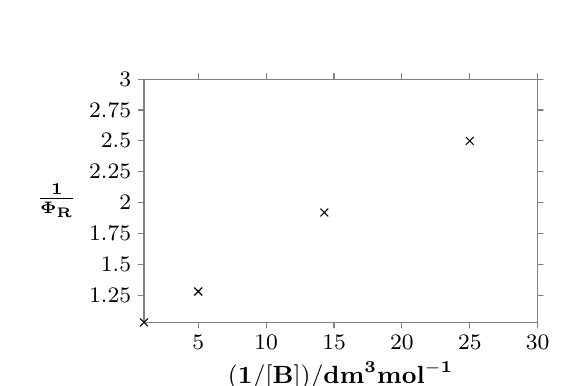
\begin{tikzpicture} 
\datavisualization [
	scientific axes={upright labels}, 
	visualize as scatter, 
	x axis = {include value = 30, label={{\(\mathbf{(1/[B])/dm^3mol^{-1}}\)}}}, 
	y axis={include value = 3, label={\(\mathbf{\frac{1}{\Phi_R}}\)}}
	]
data {
x, y
1.0, 1.03
5, 1.28
14.29, 1.92
25, 2.5
};
\end{tikzpicture}
\end{center}

\[\frac{k_1}{k_2} = 0.063\ dm^3\ mol^{-1}\]

(iii)
\begin{align*}
\frac{k_1}{k_2} &= 0.063\ dm^3\ mol^{-1}	&	k_2 &= 5\times 10^7 dm^3\ mol^{-1}s^{-1}\\
\implies k_1 &= (5\times10^7)(0.063)\\
\implies k_1 &= 3.15\times10^6\ s^{-1}\\
\tau_0 &=\frac{1}{k_F} = \frac{1}{k_1}\\
\implies \tau_0 &= \frac{1}{3.15\times10^6} = 3.17\times10^7\ s
\end{align*}

\Exercise Draw a 2-D representation of the Jablonski diagram showing energy and geometry changes and appropriately indicate the processes of absorption, internal conversion, fluorescence, intersystem crossing and phosphorescence on the diagram
\Exercise Briefly discuss the Franck-Condon principle
\Exercise Briefly discuss the Grotthus-Draper Law and Stark-Einstein Law
\Exercise Define quantum yield
\Exercise How does the value of an experimentally measured fluorescence life, \(\tau_F\), differ from the intrinsic singlet excited state lifetime, \(\tau_0\)? Briefly explain why they differ
\Exercise Briefly explain why most molecules which fluoresce in liquid solution, the fluorescence quantum yield and lifetime are independent of the absorbed wavelength

\Exercise The \(\pi\) to \(\pi^*\) transition in ethene has a \emph{high probability} of taking place. Discuss this statement with reference to the overlap of molecular orbitals in ethene

\Exercise The n \textit{n} to \(\pi^*\) transition in methanal has a \emph{low probability} of taking place. Discuss this statement with reference to the overlap of molecular orbitals in methanal.

\Exercise In the presence of \(6.67\times10^{-3}\) M concentration of a quencher, Q, the fluorescence intensity, I\(_F\), of A was diminshed to 50\% of the original intensity, I\(^0_F\). The experimentally observed fluorescence lifetime (\(\tau_F\)), was determined as \(3.35\times 10^{-10}\) s. Calculate the second order rate constant for quenching, \(k_Q\).
\[ A + Q \xrightarrow{k_Q} quenching\ products\]

\Exercise 
\Question Explain the following trends in the triplet lifetimes, \(\tau_T\), in the absence of quenching of benzene (1), naphtalene (2) and anthracene (3).\newline
\includegraphics[height=1cm]{../graphics/benzene} \hspace{1cm} \includegraphics[height=1cm]{../graphics/naphtalene} \hspace{1cm} \includegraphics[height=1cm]{../graphics/anthracene}\newline

\Question What is your understanding of the Energy Gap Law as applied to excited singlet and triplet states in an organic molecule?
\Question Why is phosphorescence seldom observed in solution but can often be seen in rigid media?
\Question Explain in terms of \(\tau_0\) the rate coefficient of internal conversion (\(k_{IC}\)) and rate coefficient of intersystem crossing (\(k_{ISC}\)) why compounds in which the lowest excited singlet state is \(n\pi^*\) in nature do not usually fluoresce strongly?
\Question Explain why \(n\pi^*\) excited systems favour a phosphorescence decay pathway as compared to \(\pi\pi^*\) systems.
\Question A molecule under examination demonstrates an emission that occurs where expected for fluorescence emission, but with a long lifetiime, \(\tau_F\), more appropriate for phosphorescence emission. If this emission is truly fluorescence, describe generally two possible mechanisms that can account for these observations
\Question Explain, with reasoning, why strong luminescence is generally only observed from the lowest singlet state (\(S_1\)) of a polyatomic hydrocarbon molecule even when excited into second (\(S_2\)) or higher singlet states (\(S_n\)). Hence indicate the reasons why the process of intersystem crossing (\(S_1/T_1\)) for organic aromatic compounds is inefficient compared to organic carbonyl compounds

\Exercise Why do the intersystem crossing rate coefficients for the halobenzenes increase with the atomic number of the incorporated halogen?

\Exercise What effects on the quantum yield of fluorescence and phosphorescence lifetime might you expect to observe as further consequence of the phenomenon above?

\Exercise Why does naphtalene (\ce{C10H8}) display a shorter phosphorescence lifetime than perdeuteronaphtalene (\ce{C10D8})

\Exercise Explain why the quantum yield of phosphorescence of benzene-\(h_6\) in a rigid glass at 80K is 0.18, but for benzene-\(d_6\) the yield is 0.24 under the same conditions

\Exercise A simple aliphatic ketone is photo-excited at 300 nm in the vapour phase. What effect would the addition of (a) oxygen and (b) xenon have on the quantum yield of phosphorescence (\(\Psi_P\))?

\Exercise What is the relationship between the quantum yield of phosphorescence (\(\Psi_P\)), the quantum efficiency of phosphorescence (\(\Theta_P\)) and the triplet quantum yield (\(\Psi_T\))?

\Exercise Molecule A is trapped in a glassy matrix at low temperature and excited to the first excited singlet state, S\textsubscript{1}. The quantum yield of fluorescence for A is 0.34, the quantum yield for triplet state, T\textsubscript{1} formation is 0.66, the quantum yield for phosphorescence is 0.024. The measured lifetime of fluorescence is 118 ns and the phosphorescence lifetime is 2.6 s.
\Question What is the rate coefficient for intersystem crossing from S\textsubscript{1} to T\textsubscript{1}?
\Question What is the rate coefficient for intersystem crossing from T\textsubscript{1} to S\textsubscript{0}?

\Exercise For molecule Z in a glassy matrix at 77K excited to the S\textsubscript{1} state, the quantum yield of fluorescence (\(\Psi_F\)) is 0.37, the triplet quantum yield (\(\Psi_T\)) is 0.63 and the quantum yield of phosphorescence (\(\Psi_p\)) is 0.027. Assuming that no internal conversion processes occur in the molecule, determine:
\Question the rate coefficient for intersystem crossing from S\textsubscript{1} to T\textsubscript{1} using the measured fluorescence lifetime, \(\tau_s\)) of 96 ns.
\Question the quantum efficiency of phosphorescence (\(\Theta_P\))
\Question the rate coefficient of phosphorescence (\(k_p\)) from T\textsubscript{1} to S\textsubscript{0} using the measured phosphorescence lifetime (\(\tau_T\)) of 1.9 s.
\Question the rate coefficient for intersystem crossing from T\textsubscript{1} to S\textsubscript{0}.

\end{ExerciseList}

\begin{Exercise}[label = ex1]
Ultraviolet radiation photolyses \ce{O3} to \ce{O2} and O in the reaction \ce{O3 + h$\nu$ -> O2 + O}

Determine the rate at which ozone is consumed by 305 nm radiation in a layer of the stratosphere of thickness 1 km. The quantum yield is 0.94 at 220K, the concentration about \(8\times10^{-9}\ mol\ dm^{-3}\), the molar absorption coefficient is 260 \(dm^3\ mol^{-1}\ cm^{-1}\), and the flux of 305 nm radiation about \(1\times 10^{14}\) photons \(cm^{-2}\ s^{-1}\).

\end{Exercise}

\begin{Answer}[ref= ex1] The rate of reaction is the rate at which ozone absorbs photons times the quantum yield. The rate at which ozone absorbs photons is the rate at which photons impinge on the ozone times the fraction of photons absorbed. That fraction is 1-T, where T is transmittance. T is related to the absorbance, A, by

\(A=-logT = \varepsilon c \ell\) so \(1-T = 1-10^{-\varepsilon c \ell}\)

\(1-T = 1-10^{-[260\ Lmol^{-1}cm^{-1} \times 8.0\times10^{-9}\ mol\ L^{-1} \times 10^5\ cm]} = 0.38\)

\end{Answer}

\begin{Exercise}[label=ex2]
the photochemical chlorination of chloroform

\ce{CHCl3 + Cl2 = CCl4 + HCl}

is believed to proceed by the following mechanism

\ce{Cl2 + h$\nu$ ->[I_a] + 2Cl}

\ce{Cl + CHCl3 ->[k_1] CCl3 +HCl}

\ce{CCl3 + Cl2 ->[k_2] CCl4 + Cl}

\ce{2CCl3 + Cl2 ->[k_3] 2CCl4}

Derive the steady state rate law for the production of carbon tetrachloride.
\end{Exercise}

\begin{Answer}[ref=ex2]
\(\frac{d[CCl_4]}{dt} = k_2[CCl_3][Cl_2] + 2k_3[CCl_3]^2[Cl_2]\)

\(\frac{d[CCl_3]}{dt} = k_1[Cl][CHCl_3] - k_2[CCl_3][Cl_2] - 2k_3[CCl_3]^2[Cl_2] = 0\)

\(\frac{d[Cl]}{dt} = 2I_a - k_1[Cl][CHCl_3] + k_2[CCl_3][Cl_2] = 0\)

Adding the two steady state expresions yields

\(I_a = k_3[CCl_3]^2[Cl_2]\)

this makes it possible to eliminate [CCl\(_3\)] from the first equation to obtain:

\(\frac{d[CCl_4]}{dt} = \frac{k_2I_a^{1/2}[Cl_2]^{1/2}}{k_3^{1/2}} + 2I_a\)
\end{Answer}

%\section{Further Reading}


\begin{frame}
\end{frame}

\end{document}

app password hjvwgltqyngsrslp

\Exercise \fbox{\parbox{.8\textwidth}{A molecule Y in a glassy matrix at 77K is excited to the S\textsubscript{1} state. The quantum yield of fluorescence (\(\Phi_F\)) is 0.32, the triple quantum yield (\(\Phi_T\)) is 0.68 and the quantum yield of phosphorescence (\(\Phi_F\)) is 0.022. The measured fluorescence lifetime (\(\tau_F\) or sometimes called \(\tau_s\)) is 94 ns, while the measured phosphorescence lifetime (\(\tau_T\)) is 1.7 s. No internal conversion processes are assumed to occur in the molecule.}}
\Answer As no internal conversion processes occur in the molecule (as stated) we assume that only processes that are taking place are \emph{fluorescence, phosphorescence and intersystem crossing}.

The best thing to do with these types of questions is to summarise the data given to you initially:\\
\begin{tabular}{l}
\(\Phi_F=0.32\)\\
\(\Phi_T=0.68\)\\
\(\Phi_p=0.022\)\\
\(\tau_s=94\) ns\\
\(\tau_T=1.7\) s
\end{tabular}\\
\includegraphics[width=.4\textwidth]{../graphics/exercise}\\
(i) Calculate the rate coefficient for intersystem crossing (\(k_{ISC}\)) from S\textsubscript{1} to T\textsubscript{1}?
\begin{itemize}
\item The competing processes to depopulate S\textsubscript{1} are intersystem crossing and fluorescence
\item \(\Phi_{ISC} = \frac{k_{ISC}}{k_{ISC} + k_F} \xrightarrow{as} \tau_s = \frac{1}{k_{ISC} + k_F} \xrightarrow{therefore} \Phi_{ISC} = k_{ISC} \cdot \tau_s \xrightarrow{re-arrange\ to\ solve\ for\ k_{ISC}} k_{ISC} = \frac{\Phi_{ISC}}{\tau_s}\)
\item As we are talking about intersystem crossing from S\textsubscript{1} tp T\textsubscript{1} then we are populating the triplet state:
\item \(\Phi_{ISC} = \Phi_T \xrightarrow{finally} k_{ISC} = \frac{\Phi_T}{\tau_s} \Rightarrow k_{ISC} = \frac{0.68}{94\times 10^{-9}} = 7.234\times10^6\ s^{-1}\)\\\medskip

(ii) Calculate the quantum efficiency of phosphorescence (\(\Theta_P\)) \\
\[\Phi_p = \Phi_T \cdot \Theta_P\]
Re-arranging to solve for \(\Theta_P\):\\
\begin{align*}
\Rightarrow \Theta_P &= \frac{\Phi_p}{\Phi_T}\\
\Rightarrow \Theta_p &= \frac{0.022}{0.68} = 0.032
\end{align*}
\end{itemize}
\medskip

(iii) Calculate the rate coefficient of phosphorescence (\(k_p\)) from T\textsubscript{1} to S\textsubscript{0}\\
\smallskip The competing processes to depopulate T\textsubscript{1} are intersystem crossing and phosphorescence
\begin{align*} \Phi_p = \frac{k_p}{k_p + k_{ISC}} \xrightarrow{as} \tau_s &= \frac{1}{k_p + k_{ISC}}\\ \xrightarrow{therefore} \Phi_p &= k_p\tau_T \\\xrightarrow{re-arranging\ to\ solve\ for\ k_p} k_p &= \frac{\Phi_p}{\tau_s}\\ \Rightarrow k_p &= \frac{0.022}{1.7} = 0.0129\ s^{-1}\end{align*}

\medskip
(iv) Calculate the rate coefficient for intersystem crossing from T\textsubscript{1} to S\textsubscript{0}\\
Again, the competing processes to depopulate T\textsubscript{1} are intersystem crossing and phosphorescence\\
\begin{align*}
\Phi_p &= \frac{k_p}{k_p + k_{ISC}}\\ \xrightarrow{re-arranging\ to\ solve\ for\ k_p} k_{ISC} &= \frac{k_p}{\Phi_p} - k_p\\ \Rightarrow k_{ISC} &= \frac{0.0129}{0.022} - 0.0129 = 0.573\ s^{-1}
\end{align*}

\begin{tikzpicture}
\datavisualization
[
scientific axes,
all axes={length=5cm},
x axis={label=x, attribute=x, min value=-2, max value=2},
y axis={label=y, attribute=y, min value=0, max value=10},
visualize as line,
]
data[read from file=test.csv, separator={\space}];
\end{tikzpicture}

\begin{tikzpicture}
\begin{axis}[height=5cm,width=5cm,
             xlabel=x,xmin=2,xmin=-2,
             ylabel=y,ymin=0,ymax=10,
             enlargelimits=0,tick align=outside]
\addplot[no markers] table[x=x,y=y] {test.csv};
\end{axis}
\end{tikzpicture}